\documentclass[onecolumn]{openhelix}
% Option "twocolumn" available, but please prioritize single-column
\usepackage{graphicx}
\usepackage{amsmath}
\usepackage{amssymb}
\usepackage{amsfonts}
\usepackage{tabularx}
\usepackage{float}
\usepackage{algorithm}
\usepackage{algorithmic}
\usepackage{utfsym}
\usepackage{array}
\usepackage{booktabs}
\usepackage{makecell}
\usepackage{wrapfig}
\usepackage{xspace}
\usepackage{nicefrac}
\usepackage{microtype}
\usepackage{multirow}
\usepackage{colortbl}
\usepackage[misc]{ifsym}
\usepackage{mathtools}
\usepackage{enumitem}

\newcommand{\huggingface}{\raisebox{-1.5pt}{
\includegraphics[height=1.05em]{assets/hf.pdf}}\xspace}
\newcommand{\hfdataset}{\raisebox{-1.5pt}{
\includegraphics[height=1.05em]{assets/db.pdf}}\xspace}
\newcommand{\github}{\raisebox{-1.5pt}{
\includegraphics[height=1.05em]{assets/github.pdf}}\xspace}

\newcommand{\WX}[1]{\textcolor{red}{WX:~#1}}
\newcommand{\ZH}[1]{\textcolor{blue}{NB:~#1}}
\newcommand{\dist}{\operatorname{dist}}
\usepackage[table]{xcolor}
\definecolor{lightgrey}{HTML}{dcdbdb}
\definecolor{lightblue}{HTML}{E8F0FE}
\definecolor{gray}{HTML}{9aa0a6}
\definecolor{lightpink}{HTML}{F48FB1}
\definecolor{lightred}{HTML}{FFCBC9}
\definecolor{lightcyan}{HTML}{80DEEA}
\newcommand{\cc}[0]{\cellcolor{lightblue}}
\newcommand{\cg}[0]{\cellcolor{lightgrey}}
\definecolor{newyellow}{HTML}{FFD94D}
\definecolor{newgrey}{HTML}{7F7F7F}
\definecolor{newpink}{HTML}{FBCDF4}
\definecolor{realworldoft}{HTML}{029533}
\definecolor{realworldsf}{HTML}{8CC46A}
\definecolor{realworldour}{HTML}{FFC715}
\newcommand{\method}{DFM-VLA}
\usepackage[most]{tcolorbox}
\tcbuselibrary{theorems}
\newtcbtheorem{finding}{Finding}{
  colback=openhelixred!5,
  colframe=openhelixred!60!black,
  fonttitle=\bfseries,
}{find}

\title{DFM-VLA: Iterative Action Refinement for Robot Manipulation via Discrete Flow Matching} 


% ORDER TBD
\author[1,2*]{Jiayi Chen}
\author[1*]{Wenxuan Song}
\author[3,4]{Shuai Chen}
\author[1]{Jingbo Wang}
% \author[5]{Yan Wang}
\author[2\dagger]{Zhijun Li}
\author[1\dagger]{Haoang Li}

\affiliation[1]{The Hong Kong University of Science and Technology (Guangzhou)}
\affiliation[2]{Harbin Institute of Technology}
\affiliation[3]{ShanghaiTech University}
\affiliation[4]{Shanghai Institute of Technical Physics, CAS}
% \affiliation[5]{Tsinghua University, AIR}

\contribution[*]{Equal Contribution}
\contribution[\dagger]{Corresponding Author}

% You can add additional metadata fields as follows
%\metadata[Code]{\url{https://github.com/openhelix-team/repo}}

\abstract{
Vision--Language--Action (VLA) models that encode actions using a discrete tokenization scheme are increasingly adopted for robotic manipulation, but existing decoding paradigms remain fundamentally limited.
Whether actions are decoded sequentially by autoregressive VLAs or in parallel by discrete diffusion VLAs, once a token is generated, it is typically fixed and cannot be revised in subsequent iterations, so early token errors cannot be effectively corrected later.
We propose \method, a discrete flow matching VLA for iterative refinement of action tokens.
\method~models a token-level probability velocity field that dynamically updates the full action sequence across refinement iterations.
We investigate two ways to construct the velocity field: an action-embedding-guided formulation and an auxiliary velocity-head formulation.
Our framework further adopts a two-stage decoding strategy with an iterative refinement stage followed by deterministic validation for stable convergence.
Extensive experiments on CALVIN, LIBERO, and real-world manipulation tasks show that \method~consistently outperforms strong autoregressive, discrete diffusion, and continuous diffusion baselines in manipulation performance while retaining high inference efficiency.
In particular, \method~achieves an average success length of 4.44 on CALVIN and an average success rate of 95.7\% on LIBERO, highlighting the value of action refinement via discrete flow matching for robotic manipulation.
}
%

\correspondence{%
\begin{tabular}[t]{@{}l@{\ }l@{}}
Jiayi Chen at & \email{1952296@tongji.edu.cn}\\
% Han Zhao at & \email{zhaohan34@westlake.edu.cn}
\end{tabular}%
}

\begin{document}

\maketitle

\section{Introduction}

\begin{figure}[t]  
    \centering
    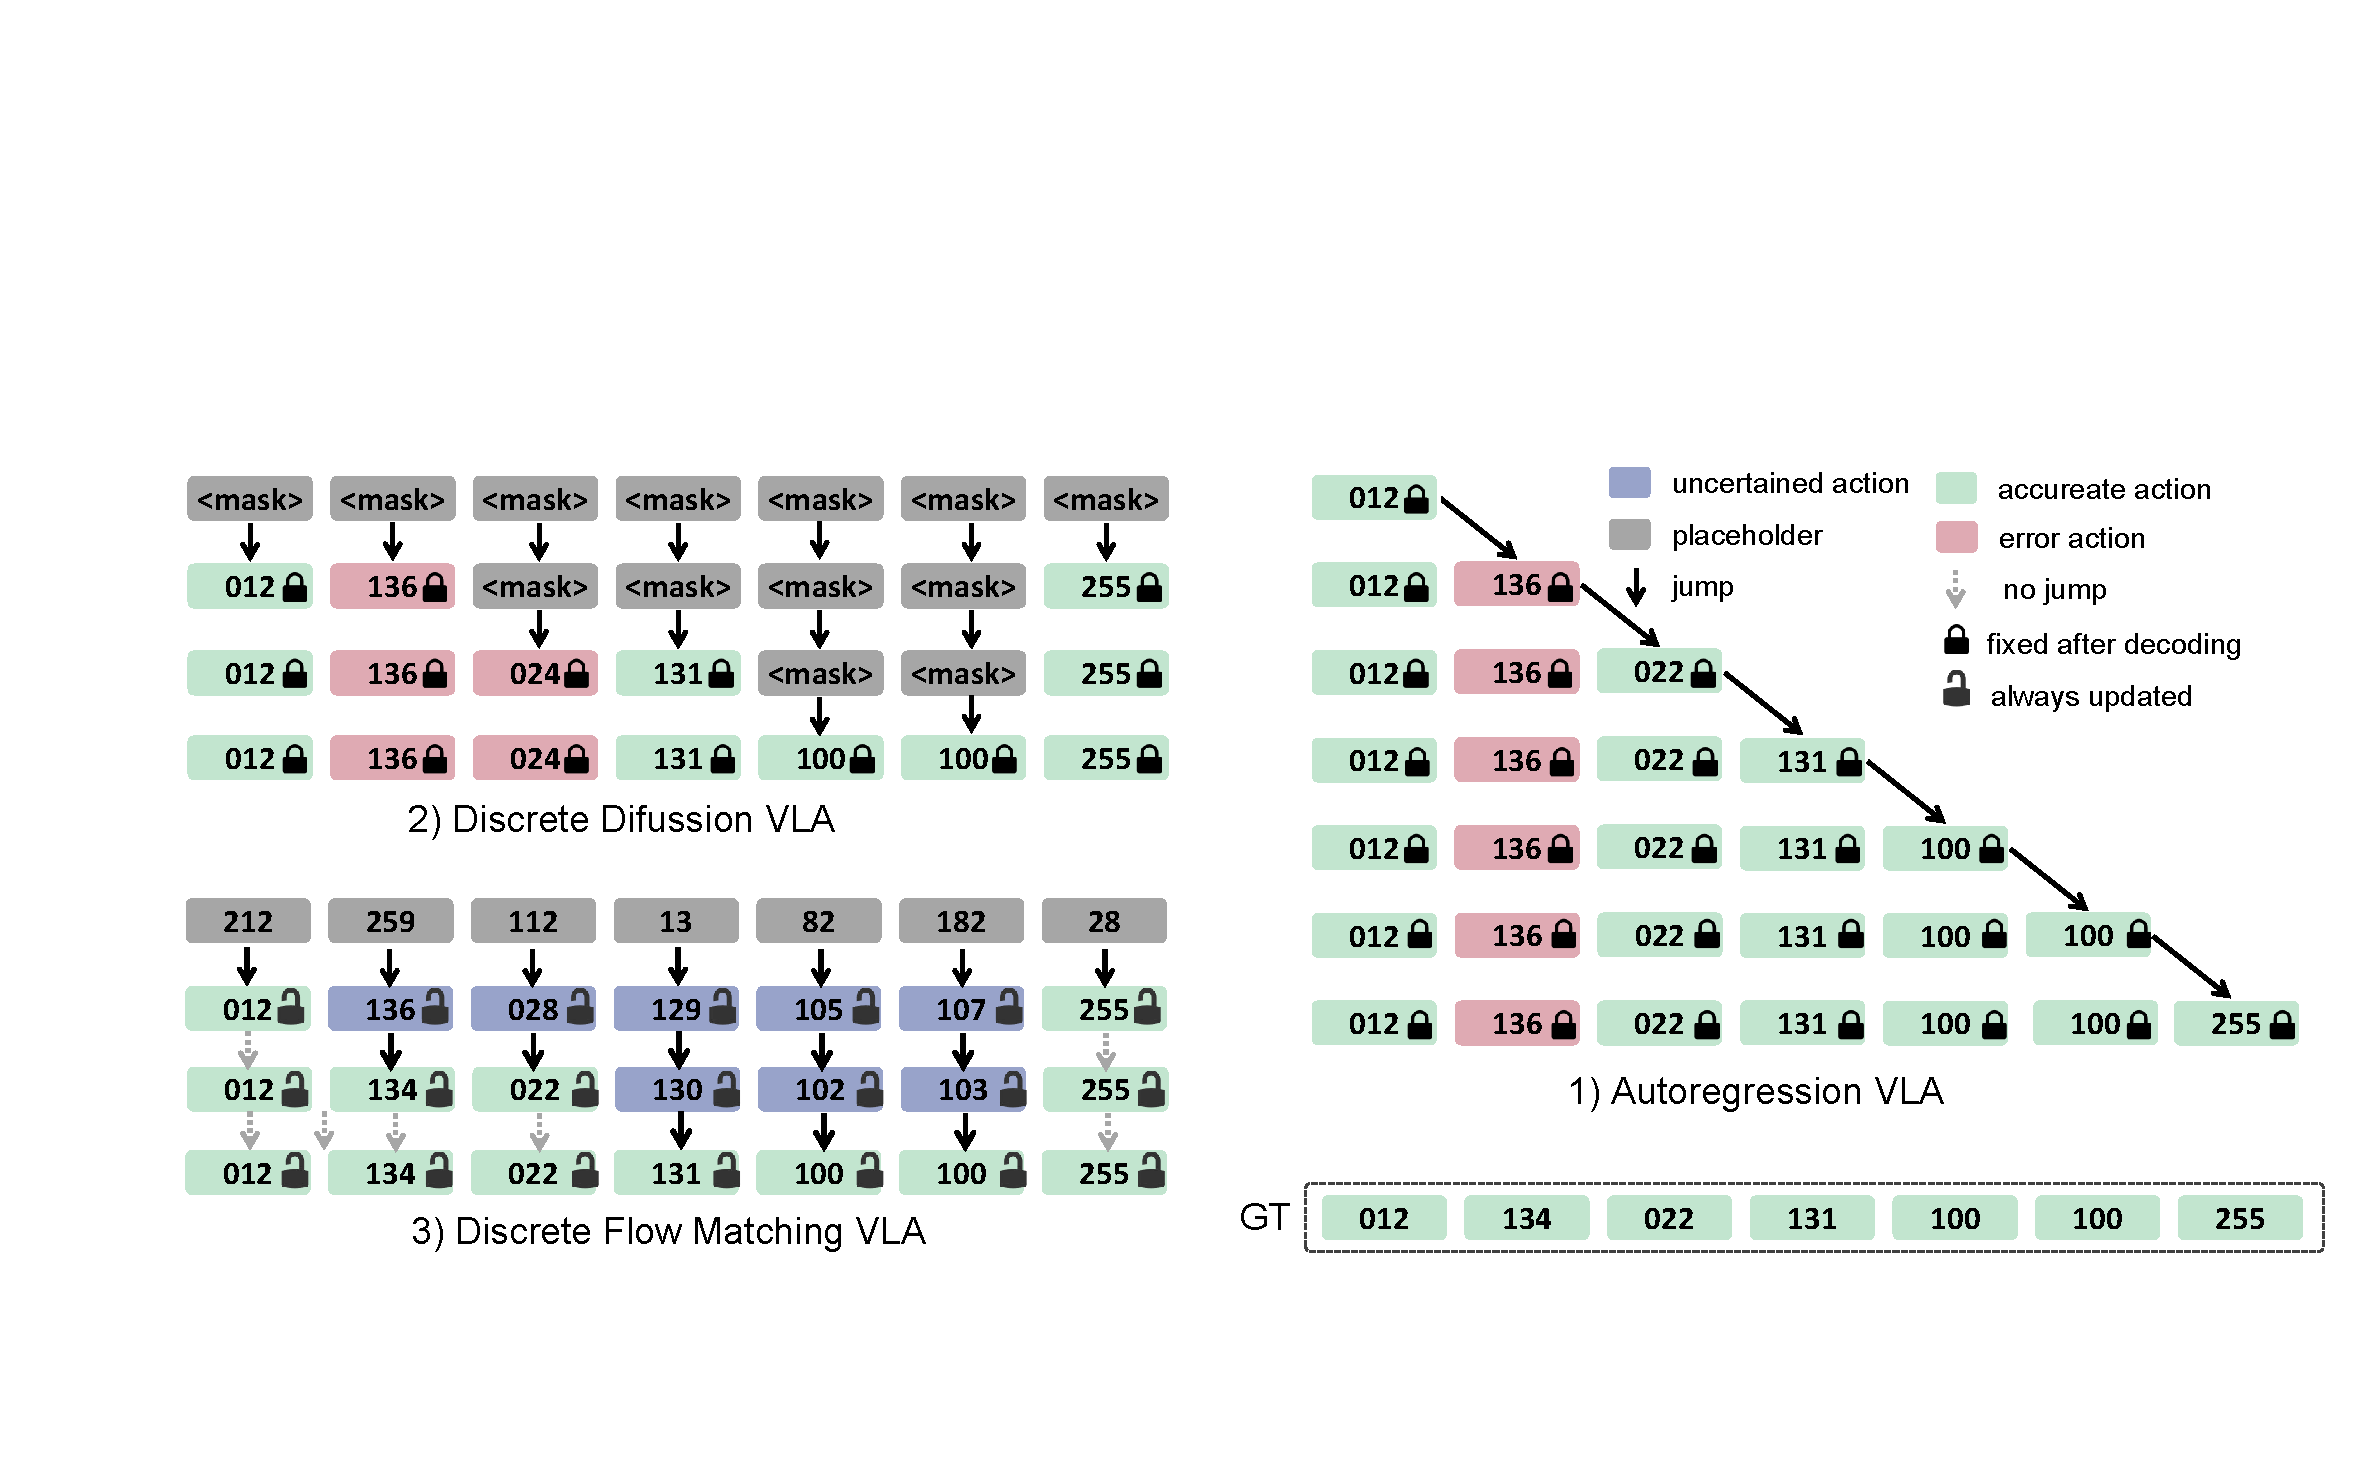
\includegraphics[width=0.98\linewidth]{figure/decode_compare.pdf} 
    \caption{Comparison of decoding paradigms. 1) Autoregressive decoding requires as many steps as the action sequence length, while 2) Discrete Diffusion enables faster generation through parallel token updates. However, both have the same limitation that once an erroneous token is produced, it cannot be corrected in later iterations.
    We refer to this phenomenon as \emph{irreversible commitment}.
    In contrast, 3) our~\method~performs full-sequence action refinement at every iteration, allowing token-level correction and improving action quality for robotic manipulation.}
    \label{fig:decode_compare} 
\end{figure}



Vision--Language--Action (VLA)~\citep{univla,Pi0,gr00t,cui2025openhelix,kim2024openvla,song2025reconvla,wang2025vlaadapter,zhong2026dualcot,yan2026svam} models have become a promising foundation for robotic manipulation, where policies map language instructions and visual observations to executable actions. 
A common and effective design is to discretize actions into tokens, which enables scalable training with Vision-Language Models (VLMs) backbones and leverages their strong capabilities in vision and language
understanding.

Most existing discrete VLA systems fall into two families. Autoregressive (AR) methods~\citep{brohan2022rt,kim2024openvla,univla} decode tokens sequentially with a next-token prediction objective. However, their inherently left-to-right decoding order makes it difficult to revise erroneous tokens once they are emitted.
Discrete diffusion (DD) methods~\citep{song2025accelerating,liang2025discrete,wen2025llada} improve parallelism and often reduce latency, but they may still produce erroneous tokens in early iterations under confidence-guided decoding (see \Cref{fig:decode_compare}).
As a result, AR and DD paradigms struggle with a shared issue in robot control: early decoding errors cannot be effectively corrected and therefore propagate through the action chunk, degrading downstream robotic task performance.
Recent Discrete Flow Matching (DFM)~\citep{wang2025fudoki,luo2025next,havasi2025edit,nguyen2025oneflow,deng2025uniform} studies on Large-Language Models (LLMs) or VLMs have demonstrated competitive performance on text reasoning and editing, as well as image and video generation, by enabling iterative token refinement and flexible generation trajectories guided by velocity field.
These advances inspire us to transfer the same refinement principle to discrete action generation for robotic control.
% Inspired by these advances, we aim to overcome the limitations of AR- and DD-based methods.

We propose \method, a VLA framework that unifies language, vision, and action in a discrete formulation, and employs a discrete action velocity field to enable holistic refinement of action sequences.
As shown in \Cref{fig:decode_compare}, instead of treating action prediction as one-shot token generation, \method~models a token-level probability velocity field and performs iterative full-sequence refinement. This formulation allows the model to repeatedly revisit previously updated positions and selectively correct uncertain tokens as context becomes more informative.
For velocity-field construction, we explore two variants, namely an action-embedding-guided formulation that defines semantically structured probability paths and derives kinetic-optimal velocities, and an auxiliary velocity head formulation that predicts velocities from model hidden states.
For decoding, we adopt a two-stage strategy consisting of an iterative refinement stage for exploration and correction, followed by a deterministic validation stage for stable convergence.

We evaluate \method~on CALVIN, LIBERO, and real-world manipulation tasks. Across benchmarks, \method~consistently improves robot manipulation quality while maintaining strong inference efficiency. Ablation studies further indicate that the proposed design is robust to key scheduler settings, training data scale, and two-stage decoding allocation.

Our contributions are summarized as follows:
\begin{itemize}
    \item We identify the \emph{irreversible commitment} problem in existing autoregressive and discrete diffusion VLA decoding, which limits token correction in robot manipulation.
    \item We propose \method, a discrete flow matching VLA framework that performs iterative full-sequence action refinement via token-level velocity.
    \item We propose two strategies for velocity field construction, namely an action-embedding-guided formulation and an auxiliary velocity head formulation, and we systematically analyze these design variants.
    \item We demonstrate strong empirical performance on CALVIN, LIBERO, and real-world tasks, with consistent gains in both action quality and inference efficiency.
\end{itemize}

\begin{figure*}[t]  
    \centering
    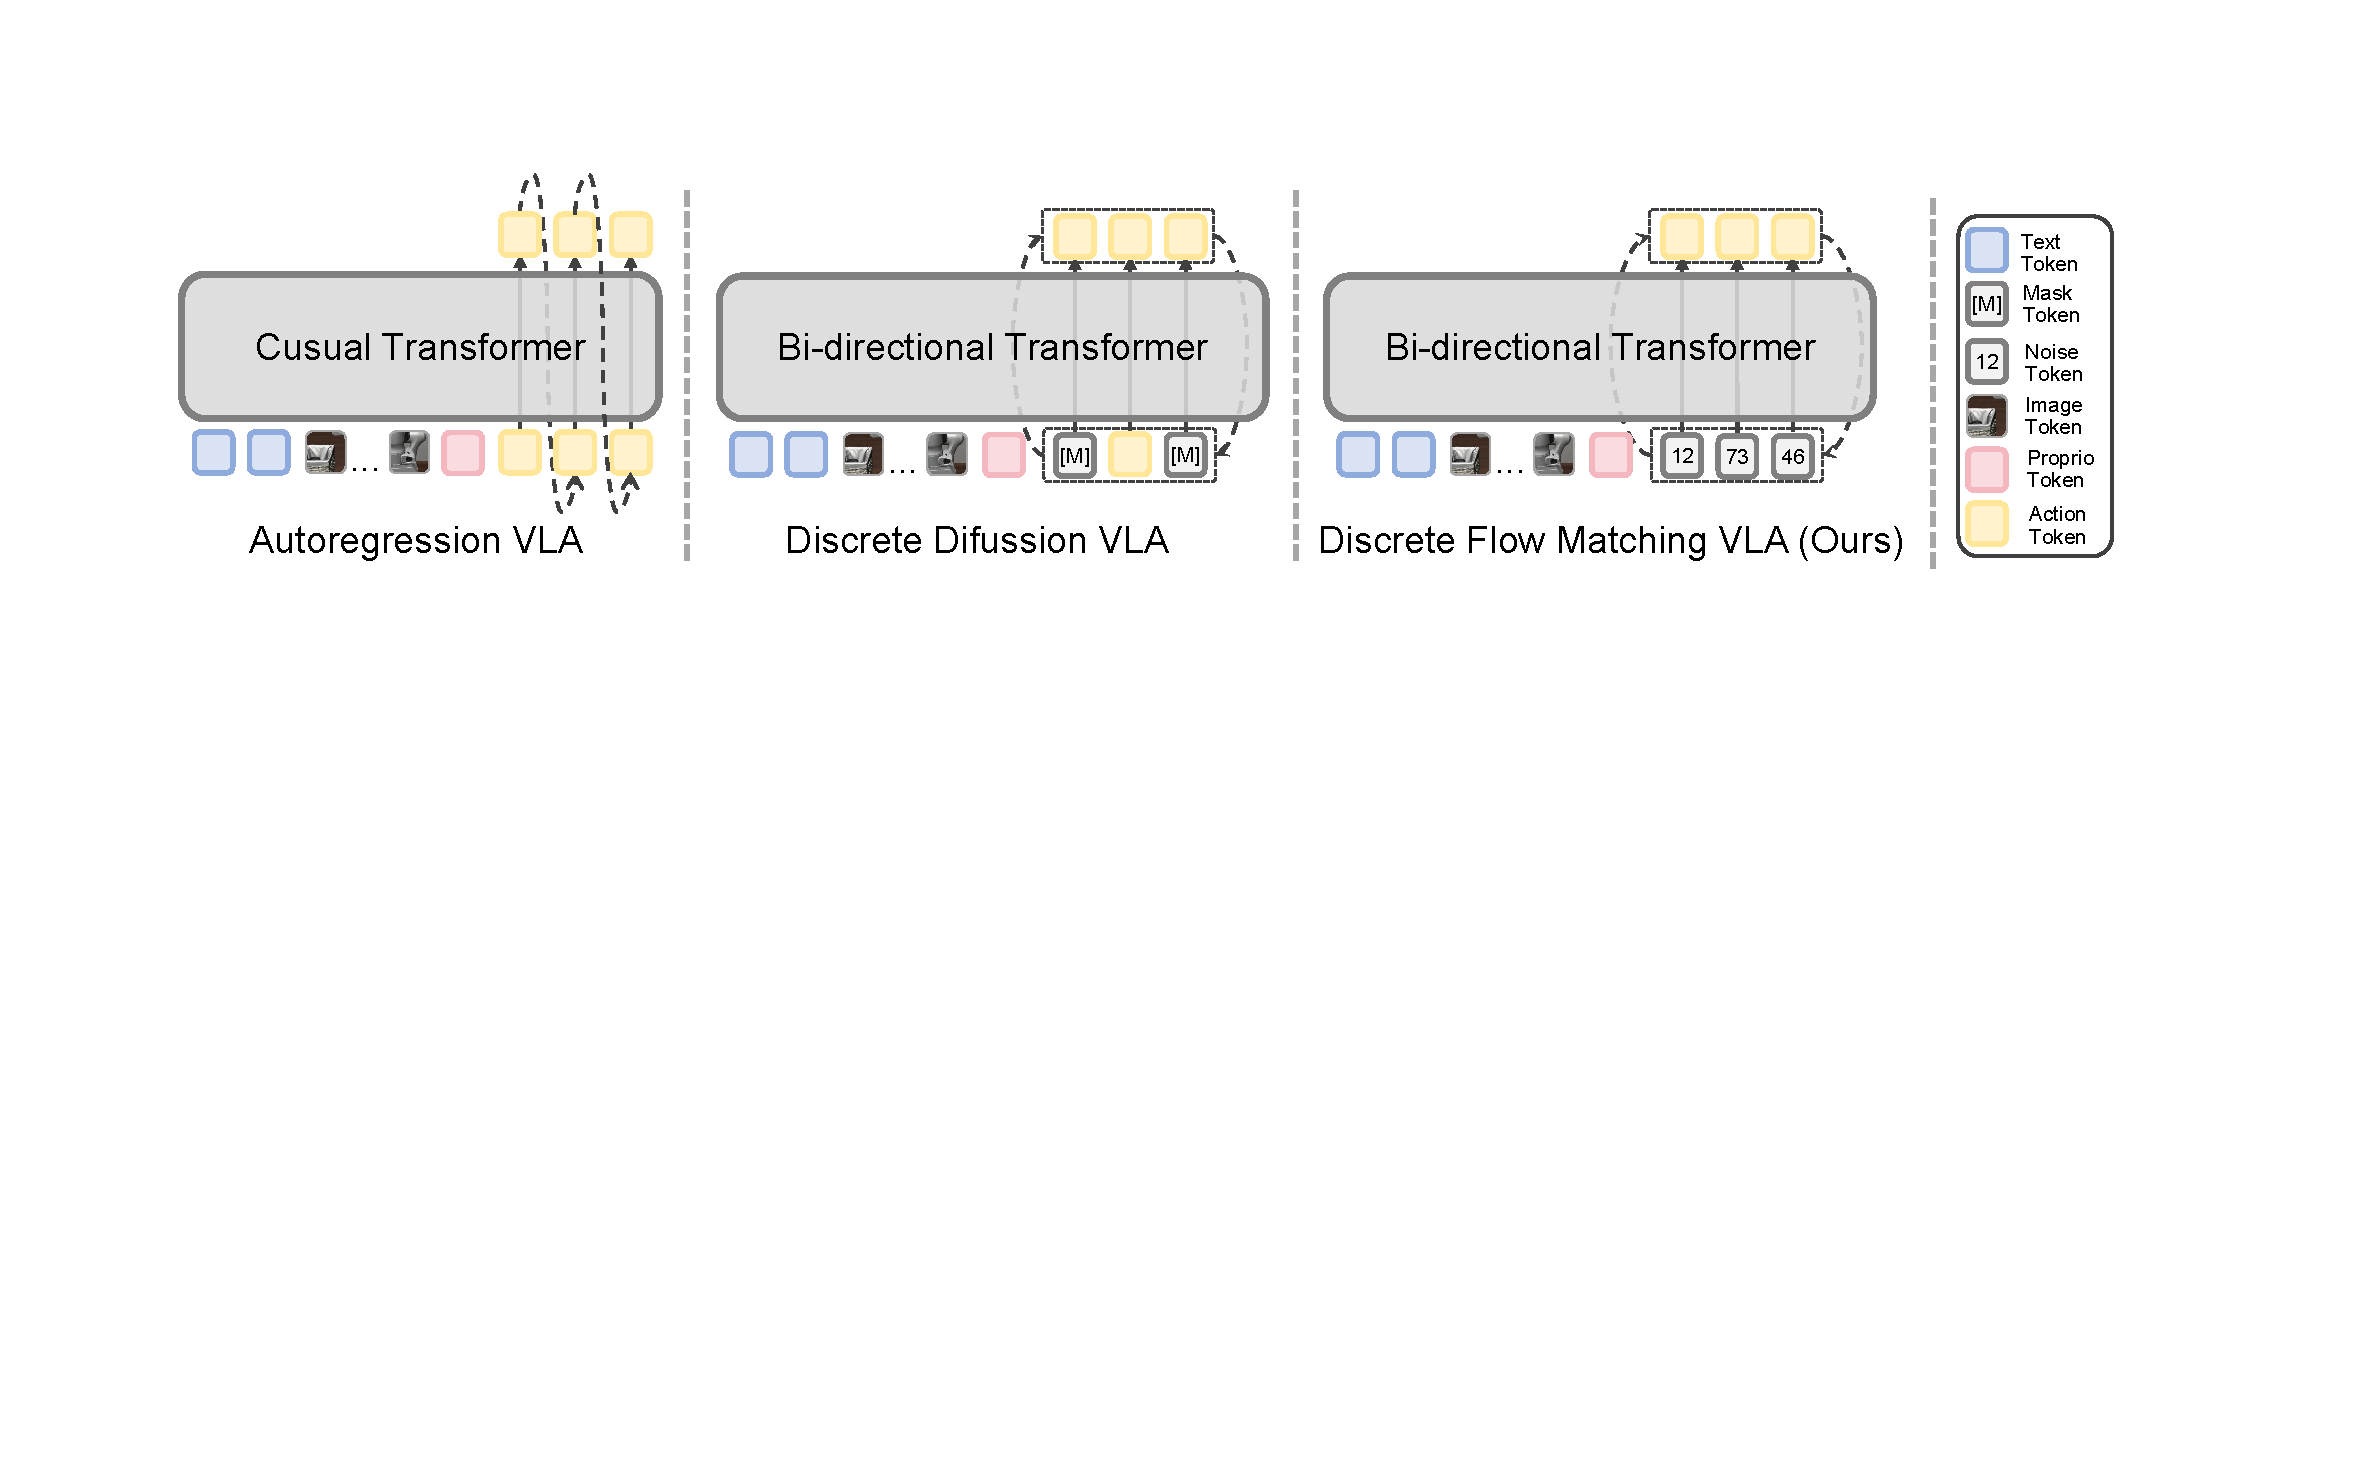
\includegraphics[width=0.98\linewidth]{figure/method_compare.pdf} 
    \caption{Comparison of three discrete VLA paradigms. 
    AR VLA uses causal attention to generate future action tokens from previously generated ones, DD-VLA decodes only masked tokens, while DFM-VLA iteratively refines tokens over the full sequence.
    }
    \label{fig:method_compare}
\end{figure*}

\section{Related Works}
\paragraph{Autoregressive VLA.}
Autoregressive VLA models(see~\Cref{fig:method_compare}) represent actions as discrete tokens, enabling LLM-style decoding and scalable training.
Representative systems include RT-1~\citep{brohan2022rt}, OpenVLA~\citep{kim2024openvla}, and LLaVA-VLA~\citep{song2026rethinking}, which unify vision, language, and action prediction under the next-to-next objective.
% Subsequent work improves perception or reasoning in discrete VLA pipelines, such as Robo-Flamingo~\citep{li2024vision}, GR-1~\citep{wu2023unleashing}, and 
ReconVLA~\citep{song2025reconvla} improves perception by reconstructing the current frame to assist discrete action generation.
Meanwhile, dynamic inference or efficiency tokenizer designs (e.g., Deer-VLA~\citep{yue2024deer} and FAST~\citep{pertsch2025fast}) target practical deployment constraints.
Methods based on vector quantization (VQ)~\citep{wang2025vq,liu2025faster,dong2026actioncodec} provide a flexible alternative by learning discrete latent representations.
UniVLA~\citep{univla} and WorldVLA~\citep{worldvla} discretize future frames to leverage dynamic visual information for action generation during both training and inference.
% 
These autoregressive models are effective but inherently sequential, which motivates our refinement alternative.
\paragraph{Discrete Diffusion VLA.}
Discrete diffusion VLA models extend dLLM-style~\citep{yu2025discrete} parallel denoising to action sequences, enabling full-attention, multi-token decoding with iterative refinement.
Representative methods differ in their corruption processes and efficiency strategies.
PD-VLA~\citep{song2025accelerating} follows a BART-style noising scheme by substituting tokens with vocabulary items and learning to reconstruct the sequence, while Discrete Diffusion VLA~\citep{liang2025discrete} and LLADA-VLA~\citep{wen2025llada} adopt BERT-style masking with a dedicated mask token~\citep{bert}.
To reduce inference cost, CEED-VLA~\citep{song2025ceed} applies consistency distillation to shrink the number of denoising steps with minimal performance loss.
On the data and modeling side, Dream-VLA~\citep{ye2025dream} scales discrete diffusion pretraining on the OXE~\citep{o2024open} datasets following OpenVLA~\citep{kim2024openvla}, and UD-VLA/dVLA~\citep{chen2025unified,wen2025dvla} incorporate visual or textual chain of thought (CoT) and jointly diffuse future frames, reasoning traces, and actions for unified perception--reasoning--action generation.
However, these dVLA methods cannot perform token-level refinement, as their updates are restricted to masked positions rather than allowing full-sequence refinement.
\paragraph{Discrete Flow Matching LLM and VLM.}
Discrete flow matching~\citep{gat2024discrete} provides a principled framework for modeling probability paths over discrete tokens, with theoretical work~\citep{shaul2024flow} establishing kinetic-optimal discrete paths and velocity formulations that generalize mask-based mixtures.
Building on these foundations, several large-scale multimodal models adopt discrete flow matching for unified understanding and generation, including Fudoki~\citep{wang2025fudoki} and Next-Omni~\citep{luo2025next}, demonstrating strong any-to-any or omnimodal capabilities.
EditFlow~\citep{havasi2025edit} introduces explicit edit operations (insertion, replacement, deletion) with learned rates to enable flexible sequence refinement, while OneFlow~\citep{nguyen2025oneflow} extends this idea to concurrent mixed-modal and interleaved generation.
URSA~\citep{deng2025uniform} further illustrates how discrete metric structures can guide token transitions in generative modeling.
We introduce discrete flow matching to the action modality, leveraging iterative refinement via a velocity field to progressively enhance action generation.
\section{Preliminary: Discrete Flow Matching}
\label{sec:preliminary}
We briefly review the key concepts and notation of discrete flow matching \citep{gat2024discrete,wang2025fudoki} that are used throughout the paper. 
DFM aims to transform a known source distribution $p(x)$ into a target data distribution $q(x)$ over a discrete space. 
We consider $x=(x^1, x^2, \ldots, x^D) \in \mathcal{S}=\mathcal{T}^D$, where $D$ is the number of discrete variables and $\mathcal{T}=[K]=\{1,2,\ldots,K\}$ is the finite alphabet of possible values.

\textbf{Probability Paths}.
Given a \emph{source distribution} \( p(x) \) and a \emph{target distribution} \( q(x) \) on a finite state space \( \mathcal{S} \), DFM defines a family of time-indexed distributions \( \{p_t(x)\}_{t \in [0,1]} \) that smoothly interpolates between \( p \) and \( q \), referred to as \emph{probability paths}.
Each \( p_t(x) \) is constructed as
$p_t(x) \coloneqq \sum_{x_1 \in \mathcal{S}} p_t(x \mid x_1) q(x_1)$,
where the conditional distribution factorizes across dimensions, i.e., $p_t(x \mid x_1) \coloneqq \prod_{i=1}^D p_t(x^i \mid x_1^i)$.
Each term \( p_t(x^i \mid x_1^i) \) interpolates between the base distribution \( p(x^i) \) and a point mass \( \delta_{x_1^i}(x^i) \), i.e., $\delta_{x_1^i}(x^i)=1$ if $x^i=x_1^i$ and $0$ otherwise. 
% We impose the boundary conditions as $p_0(x^i \mid x_1^i) = p(x^i)$ and $\quad p_1(x^i \mid x_1^i) = \delta_{x_1^i}(x^i)$,
% ensuring the path starts from the factorized distribution \( p(x) = \prod_i p(x^i) \) and ends at the target \( q(x) \).
A common choice is the \emph{mixture path} used in~\citep{gat2024discrete,havasi2025edit}, defined by a time-dependent scheduler \( \kappa_t(x_1^i) \in [0, 1] \):
\begin{equation}
p_t(x^i \mid x_1^i) = (1 - \kappa_t(x_1^i)) p(x^i) + \kappa_t(x_1^i) \delta_{x_1^i}(x^i),
\label{eq:mask_probability_path}
\end{equation}
where \( \kappa_0(\cdot) = 0 \) and \( \kappa_1(\cdot) = 1 \). The term $p_t(x^i \mid x_1^i)$ is a \emph{conditional} forward probability path that describes how the state $x^i$ evolves given $x_1^i$. 


\textbf{Probability velocities.}
%
To realize the prescribed probability path $p_{t}(x)$, we use a Continuous-Time Markov Chain (CTMC). Its dynamics are governed by a probability velocity $u_t$, also called the \emph{transition rate}, which describes how the current state $x_t$ moves toward the target state $x_1$ over time. Each token $i$ is updated independently according to
\begin{equation}\label{eq:sample}
x_{t+h}^i \sim \delta_{x_t^i}(\cdot) + h \, u_t^i(\cdot \mid x_t^i, x_1^i),
\end{equation}
where $u_t^i(\cdot \mid x_t^i, x_1^i)$ is the \emph{velocity field}, a conditional rate function that governs the flow of probability from $x_t^i$ to $x_1^i$.
%
Equation (\ref{eq:sample}) can be viewed as a small perturbation of the point mass $\delta_{x_t^i}$ scaled by the step size $h$, which models discrete state transitions in continuous time. The velocity field is central to DFM, which defines the probability-path dynamics and is the main quantity learned during training.

\section{Method}
\begin{wrapfigure}{r}{0.55\textwidth}
    \vspace{-1.2cm}
    \centering
    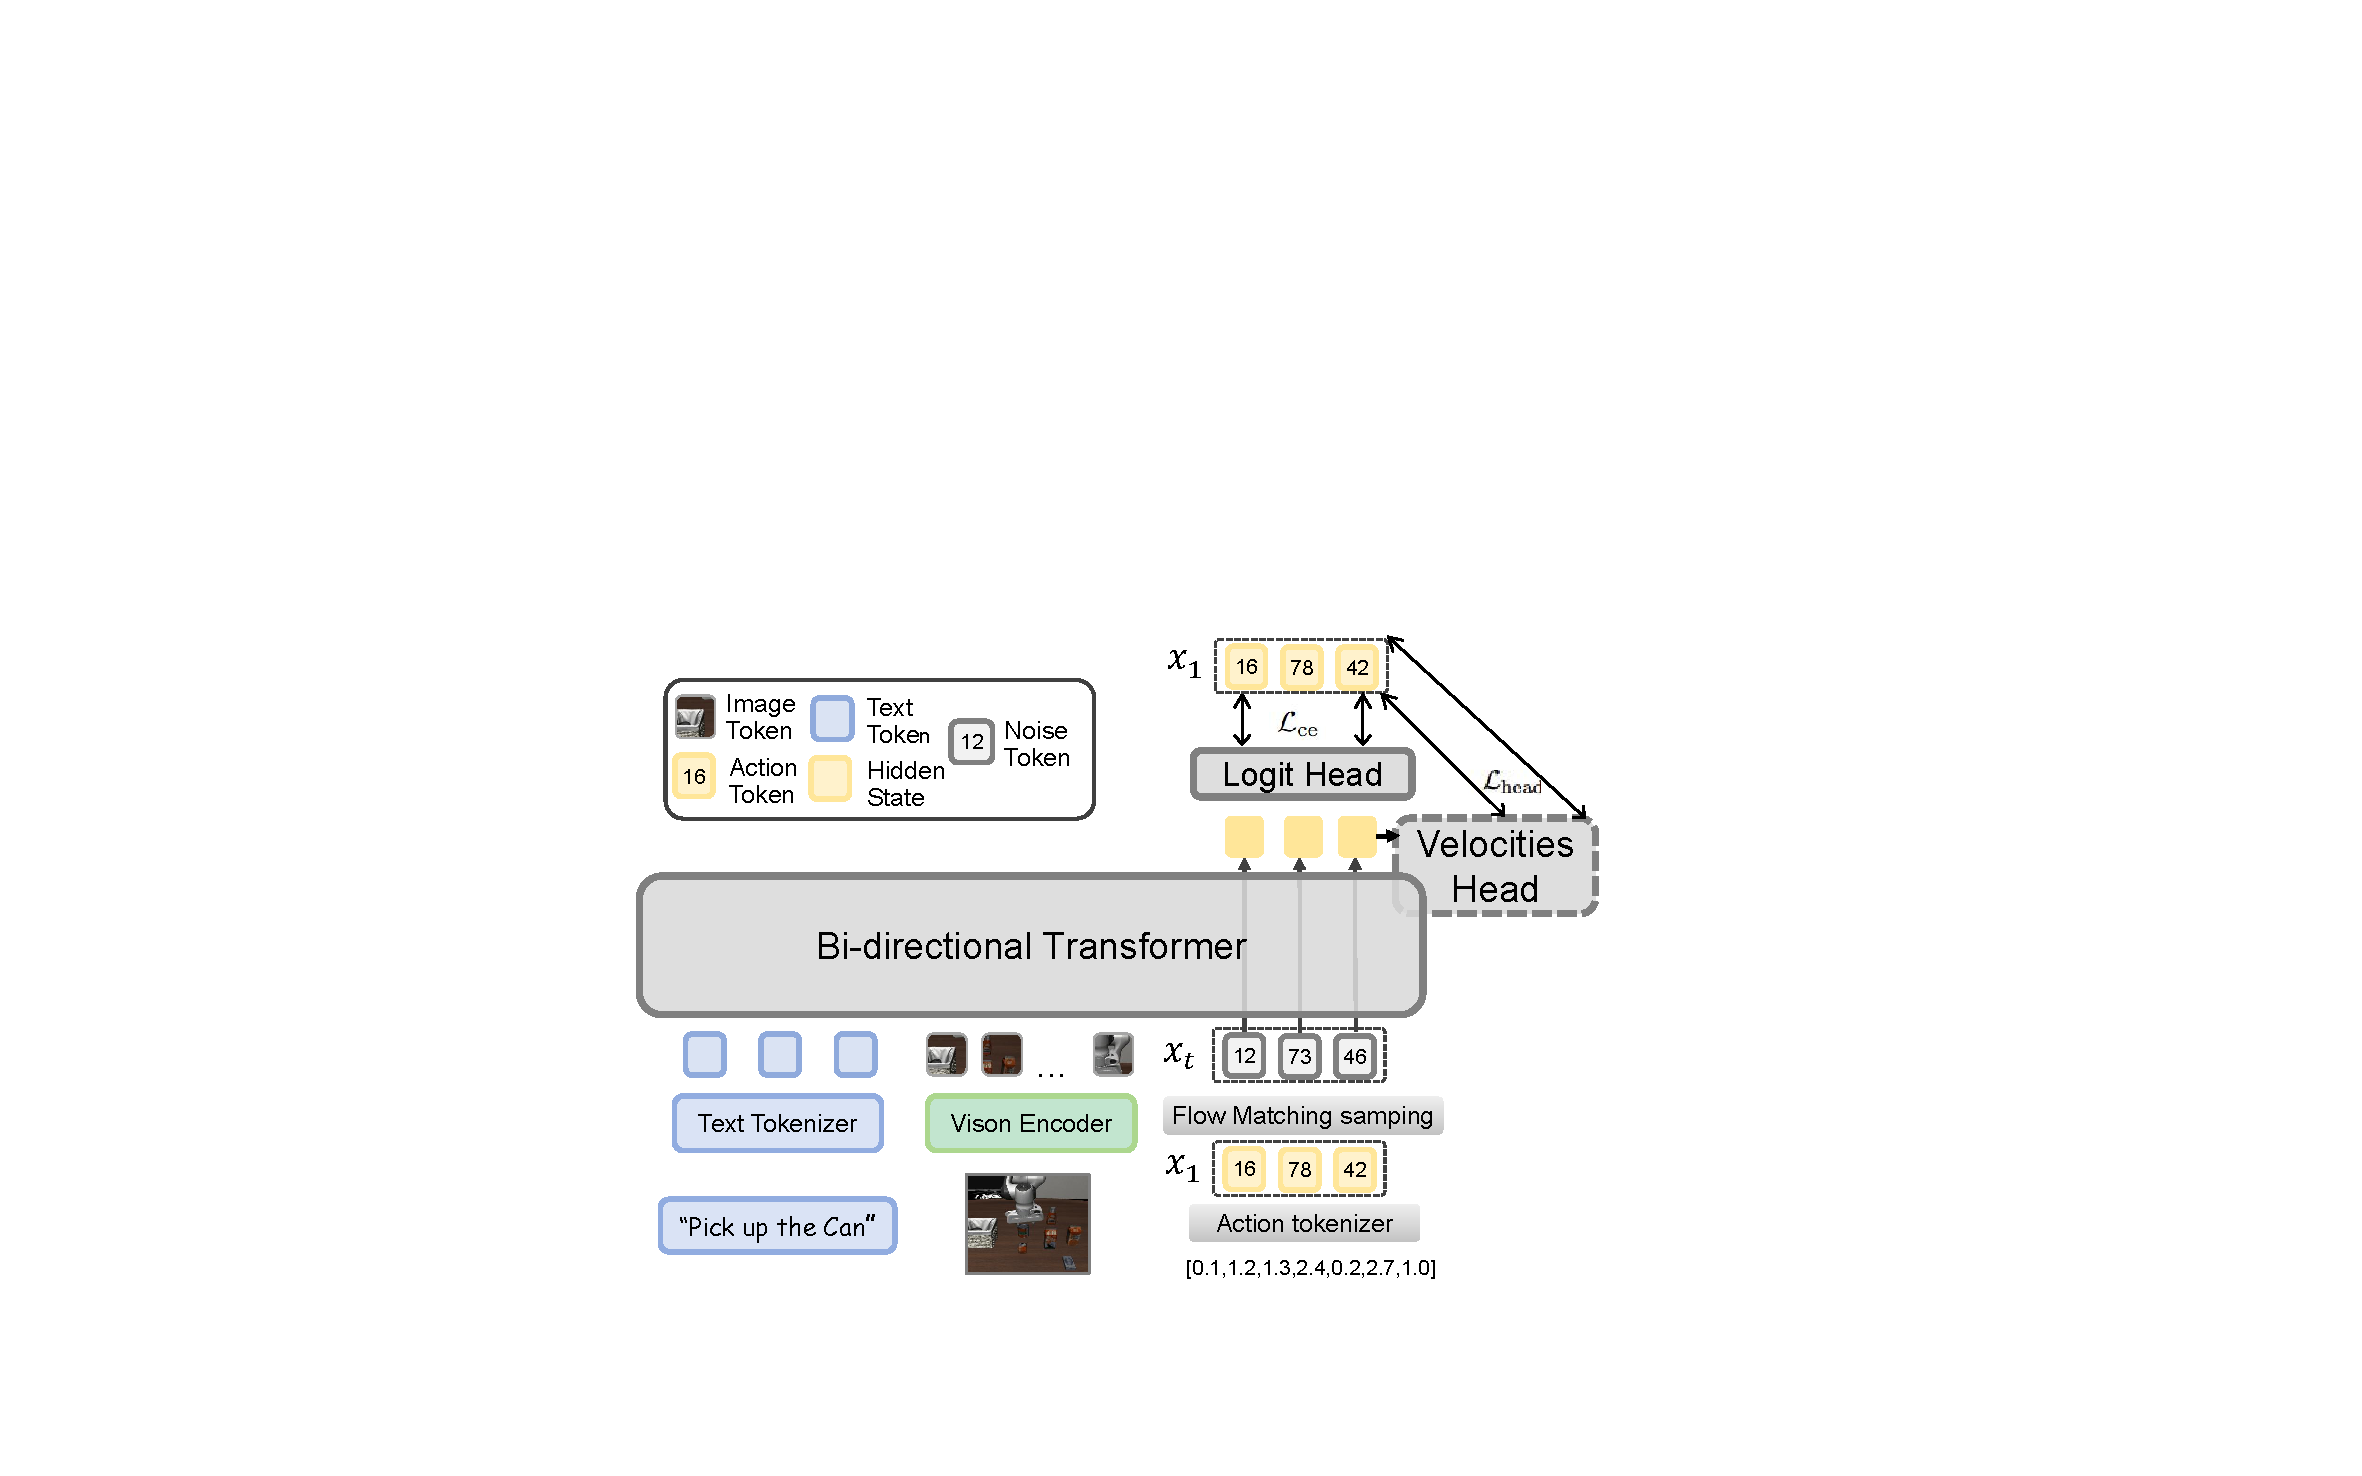
\includegraphics[width=0.99\linewidth]{figure/model.pdf} 
    \caption{Overall architecture of~\method. Given language--vision context and noised action tokens $x_t$, the model predicts clean actions $x_1$ and learns the velocity field via $\mathcal{L}_{\text{ce}}$ or ${L_\text{head}}$.}

     \vspace{-0.5cm}
    \label{fig:model_arch} 
\end{wrapfigure}
This section is organized into four parts. We first introduce the model architecture in Sec.~\ref{subsec:architecture}. We then present two velocity-field constructions: 1) an embedding-guided formulation in Sec.~\ref{sec:Embed_vel} and 2) an auxiliary velocity head formulation in Sec.~\ref{sec:head_vel}. Finally, we describe the two-stage inference procedure in Sec.~\ref{subsec:inference}.
\subsection{Architecture}
\label{subsec:architecture}
% 

As shown in \Cref{fig:model_arch}, 
DFM-VLA follows an architecture similar to UniVLA and adopts a unified discrete-token formulation for language, vision, and action modalities.
Specifically, we tokenize text using the Emu3~\citep{wang2024emu3} tokenizer, and discretize visual observations with a VQ tokenizer~\citep{zheng2022movq} using a compression ratio of 4. Both third-person and wrist-view images are represented as $25\times25=625$ tokens. For action encoding, we discretize continuous actions with FAST~\citep{pertsch2025fast} and further compress action tokens using Byte Pair Encoding (BPE), with an action vocabulary size of 1024. 
To explicitly distinguish modalities, we enclose image and action token spans with boundary markers, i.e., \texttt{boi}/\texttt{eoi} for begin/end of image and \texttt{boa}/\texttt{eoa} for begin/end of action.
In this work, we denote the discretized instruction and observations as $l$, and apply noising and prediction only to the action modality.

\subsection{Action-Embedding-Guided Velocity Modeling}
\label{sec:Embed_vel}

Building on recent advances in discrete flow matching~\citep{gat2024discrete,wang2025fudoki,deng2025uniform}, we parameterize the probability path in a metric-induced form. 
Specifically, let \( d : \mathcal{T} \times \mathcal{T} \to \mathbb{R}_{\geq 0} \) be a distance such that \( d(x^i, x_1^i) = 0 \) if and only if \( x^i = x_1^i \), where \( d(\cdot, \cdot) \) is measured in the action token embedding space. We define the conditional path as
\begin{equation}
p_t(x^i \mid x_1^i) = \mathrm{softmax}\big( -\beta_t \cdot d(x^i, x_1^i) \big),
\label{eq:diffusion-softmax}
\end{equation}
where $\beta_t:[0,1] \to \mathbb{R}_{\ge 0}$ is a monotonic schedule with boundary conditions $\beta_0 = 0$ and $\beta_1 = \infty$. We instantiate it as
\begin{align}\label{eq:beta_t}
\beta_t = c \left(\dfrac{t}{1-t}\right)^\alpha, \qquad t \in [0,1),
\end{align}
where $c>0$ and $\alpha>0$ control how fast probability mass concentrates toward the target token over time. 
% Compared with the mask-based path in Eq.~\ref{eq:mask_probability_path}, 
This formulation preserves semantic neighborhood structure such that tokens closer to $x_1^i$ receive larger probability as $t \to 1$.

Given this prescribed path, we adopt the kinetic-optimal velocity obtained by minimizing transport energy under the flow constraints~\citep{wang2025fudoki,deng2025uniform,luo2025next}:
\begin{equation}
\begin{aligned}
u_t^i(x^i, z \mid x_1) = p_t(x^i \mid x_1^i) \, \dot{\beta}_t \, [ d(z^i, x_1^i) - d(x^i, x_1^i) ]_+
\end{aligned} 
\label{eq:ko-verlocity}
\end{equation}
where $[\cdot]_+ = \max\{\cdot, 0\}$,  $z^i$ is token in the vocabulary $\mathcal{T}$, and $\dot{\beta}_t$ is the derivative of $\beta_t$ w.r.t. $t$. This velocity moves probability mass from $z^i$ to $x^i$ only when $x^i$ is closer to $x_1^i$ than $z^i$, yielding a monotonic refinement process toward the clean target token.

\textbf{Training.}  
Given language--vision context $l$ and corrupted action tokens $x_t$, the model predicts the target action sequence $x_1$ by outputting per-position categorical logits. We optimize the expected cross-entropy:
\begin{equation}
\label{eq:training_loss}
\mathcal{L_\text{ce}} = \mathbb{E}_{t \sim \mathcal{U}[0,1],\, {x}_1, {x}_t}
\left[ -\log p_{1 \mid t}\left( {x}_1 \mid {x}_t, {l}\right) \right].
\end{equation}
where $p_{1|t}^{\theta}(\cdot \mid x_t, l)$ denotes the predicted categorical distribution of the model at each action token position.

\subsection{Modeling Velocities by Additional Head}
\label{sec:head_vel}
% inspire by editflow，我们探索了构建速度场的另一种形式，editflow通过额外的速度头同时建模插入替换以及删除的三种速度场，我们只保留替换操作，因为相对文本而言，动作token的长度设计好的，相对于动作预测任务单独建模动作token的替换速率场就可以，
Drawing inspiration from EditFlow~\citep{havasi2025edit}, which employs additional velocity heads to model three types of edit operations—\emph{insertion}, \emph{replacement}, and \emph{deletion}—we explore an alternative formulation for velocity-field construction. We retain only the \emph{replacement} operation, because the action token sequence length is predefined by our action chunk design and the three operations are fundamentally equivalent under appropriate reformulation~\citep{nguyen2025oneflow,havasi2025edit}. 
% Consequently, for action prediction, modeling only a replacement velocity field is sufficient.
Concretely, given noisy action tokens $x_t$ and context $l$, the backbone first produces hidden states, and the additional velocity head then maps these hidden states to replacement velocities:
\begin{equation}
\label{eq:head-verlocity}
h_t = f_{\theta}(x_t, l), \qquad
u_t^{\theta}(\cdot \mid x_t) = u_t^{\text{head}}(h_t),
\end{equation}
where $f_{\theta}$ denotes the backbone network and $u_t^{\text{head}}$ denotes the velocity prediction head.
\begin{equation}
\small
\mathcal{L_\text{head}}
=
\mathbb{E}_{t \sim \mathcal{U}[0,1],\, {x}_1, {x}_t}
\left[
\sum_{x\neq x_t} u_t^\theta(x\mid x_t)
-
\sum_{i=1}^{N}\mathbf{1}_{[x^i_t\neq x^i_1]}\,
% \frac{\dot{\kappa}_t}{1-\kappa_t}\,
\log u_t^\theta\!\left(x^i\mid x^i_t\right)p_{1 \mid t}\left( {x}^i_1 \mid {x}^i_t, {l}\right)
\right].
\end{equation}
% \begin{equation}
% \mathcal{L_\text{head}}
% =
% \mathbb{E}_{t \sim \mathcal{U}[0,1],\, }
% \left[
% \sum u_t^\theta(x\mid x_t)
% -
% \sum_{i=1}^{N}\mathbf{1}_{[x^i_t\neq x^i_1]}\,
% % \frac{\dot{\kappa}_t}{1-\kappa_t}\,
% \log u_t^\theta\!\left(x^i\mid x^i_t\right)p_{1 \mid t}\left( {x}^i_1 \mid {x}^i_t, {l}\right)
% \right].
% \end{equation}
\noindent Here, \(\mathbf{1}_{[x_t^i \neq x_1^i]}\) is an indicator that equals 1 only when the current token differs from the target token, so the update loss is applied only to positions that still need refinement.
As shown in~\Cref{fig:velocity_field_compare}, the embedding-guided objective (\(\mathcal{L}_{\text{ce}}\)) converges faster and achieves better final performance than the head-based objective (\(\mathcal{L}_{\text{head}}\)). Unless otherwise specified, all experiments use the embedding-guided setting.

\subsection{Inference}
\label{subsec:inference}
\begin{figure*}[t]  
    \centering
    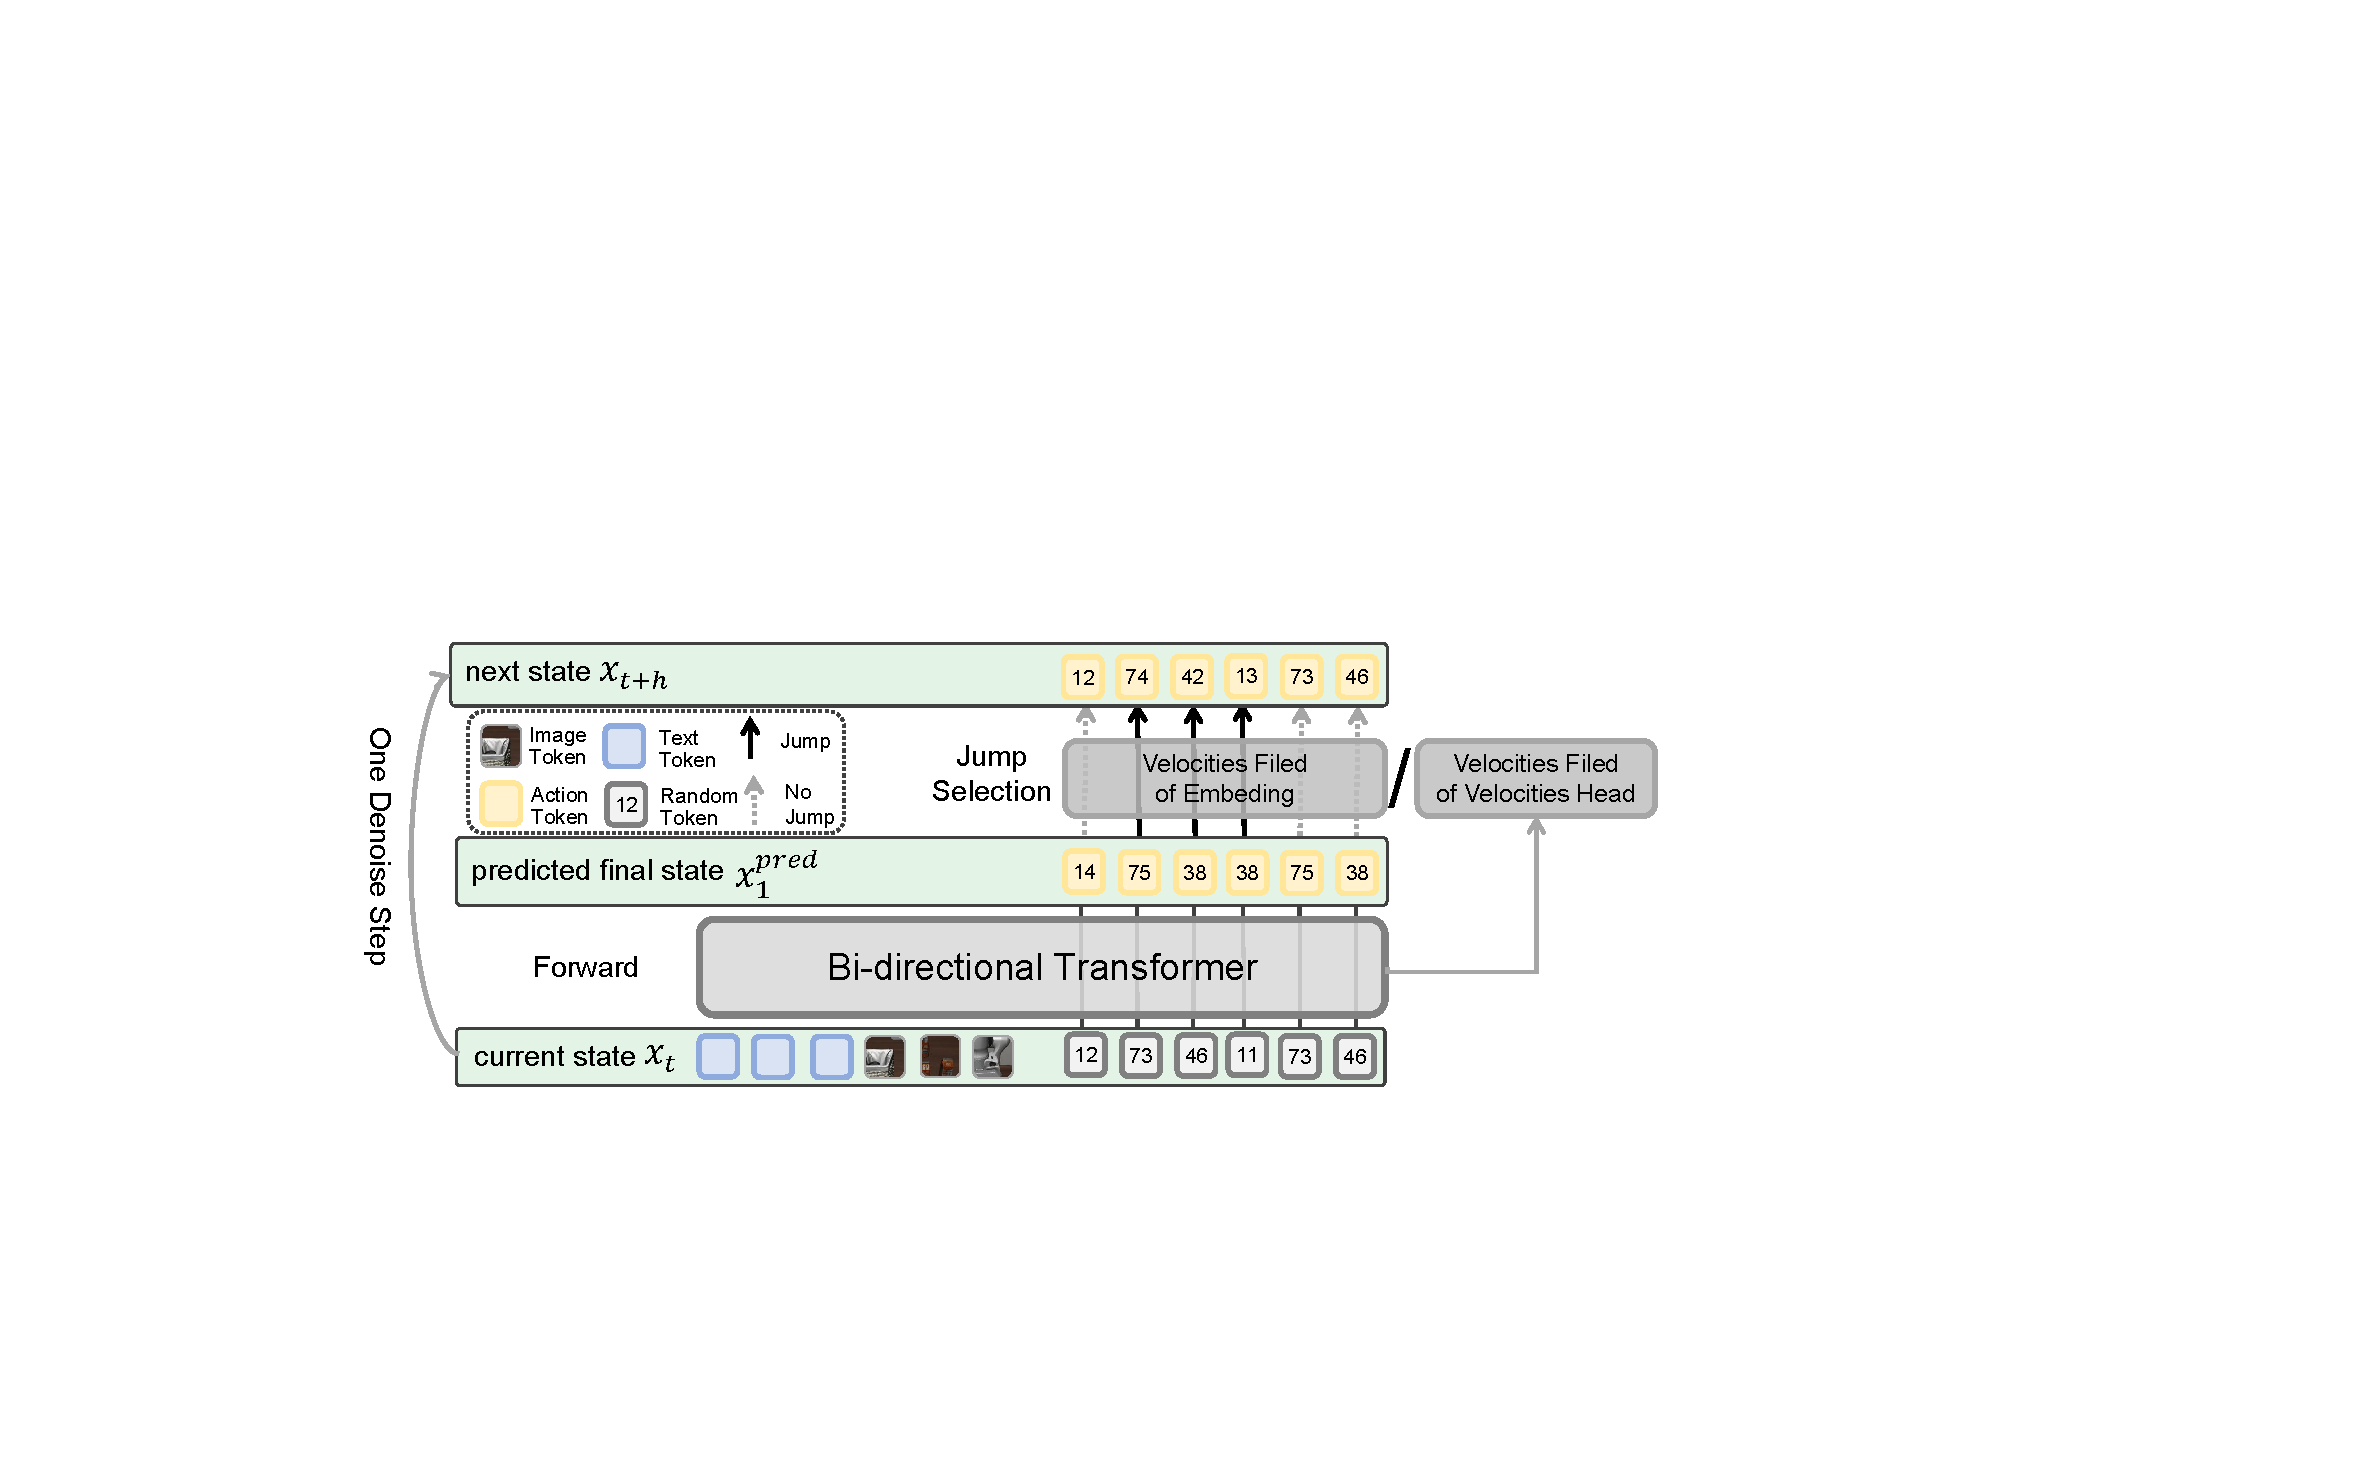
\includegraphics[width=0.98\linewidth]{figure/inference_one_step.pdf} 
    \caption{Visualization of a single decoding step in the iterative refinement stage. After predicting final state $x^\text{pred}_1$, the model does not directly output final action tokens. Instead, it constructs a velocity field to compute transition rates and selectively updates tokens to next state $x_{t+h}$ at each step.}
    \label{fig:inference} 
\end{figure*}
We perform inference in two stages: an iterative refinement stage followed by a deterministic validation stage, with $T_{\mathrm{fine}}$ and $T_{\mathrm{val}}$ decoding steps, respectively.

In the iterative refinement stage, we employ an Euler discretization of the continuous-time Markov chain (CTMC) process \( (x_t)_{0 \leq t \leq 1} \), following the approach in\citep{deng2025uniform}. As illustrated in \Cref{fig:inference}, for each coordinate \(i\) and each step from \(t\) to \(t+h\), we perform:
\begin{itemize}[itemsep=0pt, parsep=0pt, leftmargin=2em]
  \item Sample \( x_1^i \sim p_{1|t}^i(\cdot \mid x_t, l) \) from the model;
  \item Compute the total outgoing rate \( \lambda^i = \sum_{x^i \neq x_t^i} u_t^i(x^i, x_t^i \mid x_1^i) \) using Eq.~\ref{eq:ko-verlocity} or Eq.~\ref{eq:head-verlocity};
  \item Draw \( Z^i_{\text{change}} \sim U[0,1] \);
  \item Update \( x_{t+h}^i \): if \( Z^i_{\text{change}} \leq 1 - e^{-h\lambda^i} \), sample from \( \frac{u_t^i(\cdot, x_t^i \mid x_1^i)}{\lambda^i}(1-\delta_{x_t^i}(\cdot)) \); otherwise keep \( x_{t+h}^i=x_t^i \).
\end{itemize}
Here, \(\lambda^i\) is the total transition intensity out of the current token \(x_t^i\), so the jump probability \(1-e^{-h\lambda^i}\) increases with \(\lambda^i\). When a jump occurs, normalized rates favor states with larger velocity flow, which typically move the token closer to the predicted clean state \(x_1^i\). Repeating this process over time enables iterative correction across the full sequence.
Compared with mask-based discrete diffusion methods~\citep{yedreamVLA}, this decoding scheme allows previously updated tokens to be revised again in later iterations, rather than being permanently fixed after being predicted.
% \looseness=-1

\noindent
During the validation stage, we adopt a greedy decoding strategy to improve stability in the final refinement steps. 
In the final $T_{\mathrm{val}}$ decoding steps, we disable stochastic jumps and switch to greedy decoding,
\begin{equation}
    x_{t+h} = \arg\max \mathrm{softmax}(p_{1|t}(\cdot | x_t)),
\end{equation}
% where $\hat{y}_t$ is the model output logits. 
This hybrid design preserves exploratory refinement in earlier iterations while enforcing deterministic convergence near the end, leading to more stable validation-time trajectories and improved reproducibility. 
The concise two-stage decoding procedure is summarized in \Cref{alg:two_stage_sampling}.

\begin{algorithm}[b]
\caption{Two-Stage Decoding of \method}
\label{alg:two_stage_sampling}
\begin{algorithmic}[1]
\STATE \textbf{Input:} predictor $p_\theta$, context $l$, steps $T_{\mathrm{fine}},T_{\mathrm{val}}$, action vocabulary $\mathcal{V}$
\STATE Sample $x_0 \sim \mathrm{Uniform}(\mathcal{V})$; set $T \gets T_{\mathrm{fine}} + T_{\mathrm{val}}$
\FOR{$k=1$ to $T$}
    \STATE $t \gets (k-1)/T$, $h \gets 1/T$
    \STATE $\hat{x}_1 \sim p_\theta(\cdot \mid x_t, l)$
    \IF{$k \le T_{\mathrm{fine}}$}
        \STATE Compute velocity $u_t$ from $\hat{x}_1$ (Eq.~\ref{eq:ko-verlocity} or Eq.~\ref{eq:head-verlocity})
        \STATE Update $x_{t+h}$ by a  CTMC Euler step
    \ELSE
        \STATE Update $x_{t+h} \gets \arg\max p_\theta(\cdot \mid x_t, l)$
    \ENDIF
\ENDFOR
\STATE \textbf{Output:}  action sequence $x_1$
\end{algorithmic}
\end{algorithm}

\noindent
\textbf{Adaptive KV Caching.}
Following the dynamic caching strategy of FAST-dLLM~\citep{wu2025fast} on discrete diffusion decoding, we exploit the fact that many tokens exhibit only minor KV-state changes across iterative denoising steps of DFM. 
We keep the instruction and observation KV caches largely fixed throughout inference, while adaptively updating the action-side cache based on the cosine similarity between current and cached value features.
Combined with the parallel refinement of \method, this dynamic KV reuse yields a 2.4$\times$ latency speedup over autoregressive decoding while preserving task performance (see~\Cref{tab:efficiency_main}).


\begin{table*}[t]
    \footnotesize
    % \renewcommand{\arraystretch}{1.2}
    \setlength{\tabcolsep}{5pt}
    \centering
    \caption{\textbf{Comprehensive Evaluation of Long-Horizon Robotic Manipulation on the CALVIN Benchmark.} UniVLA$^{*}$ denotes the variant without historical frames for fair comparison.}
    \resizebox{\textwidth}{!}{%
    \begin{tabular}{l l c c c c c c}
        \toprule
        \multirow{2}{*}{\textbf{Method}}  & \multirow{2}{*}{\textbf{Task}} & \multicolumn{5}{c}{\textbf{Tasks Completed in a Row}} & \textbf{Avg. Len $\uparrow$} \\
        \cmidrule(lr){3-7}
        &  & 1 & 2 & 3 & 4 & 5 & \\
        \midrule
        MCIL~\citep{lynch2020language} & ABCD$\rightarrow$D &0.373 & 0.027 & 0.002 & 0.000 & 0.000 & 0.40\\
        RT-1~\citep{brohan2022rt}  & ABCD$\rightarrow$D & 0.844 & 0.617 & 0.438 & 0.323 & 0.227 & 2.45 \\
        Robo-Flamingo~\citep{li2024vision} & ABCD$\rightarrow$D & 0.964 & 0.896 & 0.824 & 0.740 & 0.660 & 4.09 \\
        Deer~\citep{yue2024deer} & ABCD$\rightarrow$D & 0.982 & 0.902 & 0.821 & 0.759 & 0.670 & 4.13 \\
        GR-1~\citep{wu2023unleashing}  & ABCD$\rightarrow$D & 0.949 & 0.896 & 0.844 & 0.789 & 0.731 & 4.21 \\
        ReconVLA~\citep{song2025reconvla}  & ABCD$\rightarrow$D & 0.980 & 0.900 & 0.845 & 0.785 & 0.705 &  4.23 \\
        UniVLA$^{*}$~\citep{univla}  & ABCD$\rightarrow$D & 0.948 & 0.906 & 0.862 & 0.834 & 0.690 & 4.26 \\
        MODE~\citep{reussefficient}  & ABCD$\rightarrow$D & 0.971 & 0.925 & 0.879 & 0.835 & 0.779 & 4.39 \\
        UP-VLA~\citep{zhang2025upvla}  & ABCD$\rightarrow$D & 0.962 & 0.921 & 0.879 & 0.842 & \textbf{0.812} & 4.42 \\
        % MDT~\citep{reuss2024multimodal}  & ABCD$\rightarrow$D & 0.986 & 0.958 & 0.916 & 0.862 & 0.801 & 4.52 \\
        % RoboVLMs~\citep{li2024towards} & ABCD$\rightarrow$D & 0.967 & 0.930 & 0.899 & 0.865 & 0.826 & 4.49 \\
        \rowcolor[gray]{0.9} \textbf{\method+Head}  & ABCD$\rightarrow$D & 0.968 & 0.928 & 0.880 & \textbf{0.864} & 0.776 & 4.42\\
        \rowcolor[gray]{0.9} \textbf{\method+Embed}  & ABCD$\rightarrow$D & \textbf{0.976} & \textbf{0.944} & \textbf{0.892} & 0.844 & 0.780 & \textbf{4.44}\\

        \bottomrule
    \end{tabular}
    }
    \label{tab:calvin_results}
    \vspace{-0.3cm}

\end{table*}
\begin{table*}[t]
\setlength{\tabcolsep}{10pt}
\footnotesize
\centering
\caption{\textbf{Evaluation and comparison on the LIBERO benchmark.}}
\resizebox{\textwidth}{!}{%
\begin{tabular}{lcccc|c}
\toprule
\textbf{Method} & \textbf{Spatial} & \textbf{Object} & \textbf{Goal} & \textbf{Long} & \textbf{Average} \\
\midrule
% DP*~\citep{chi2023diffusion}         & 78.3\% & 92.5\% & 68.3\% & 50.5\% & 72.4\% \\
Octo~\citep{octo_2023}               & 78.9\% & 85.7\% & 84.6\% & 51.1\% & 75.1\% \\
% OpenVLA~\citep{kim2024openvla}       & 84.9\% & 88.4\% & 79.2\% & 53.7\% & 76.5\% \\
SpatialVLA~\citep{qu2025spatialvla}  & 88.2\% & 89.9\% & 78.6\% & 55.5\% & 78.1\% \\
CoT-VLA~\citep{zhao2025cot}          & 87.5\% & 91.6\% & 87.6\% & 69.0\% & 81.1\%\\
WorldVLA~\citep{worldvla}          & 87.6\% &  96.2\% & 83.4\% & 60.0\% & 81.8\%\\
ThinkAct~\citep{huang2025thinkact}          & 88.3\% &  91.4\% & 87.1\% & 70.9\% & 84.4\%\\
$\pi_0$-FAST~\citep{pertsch2025fast} & 96.4\% & 96.8\% & 88.6\% & 60.2\% & 85.5\% \\
MolmoAct~\citep{lee2025molmoact}          & 87.0\% &  95.4\% & 87.6\% & 77.2\% & 86.6\%\\
FlowVLA~\citep{zhong2025flowvla}          & 93.2\% &  95.0\% & 91.6\% & 72.6\% & 88.1\%\\
DreamVLA~\citep{dreamvla25}          & \textbf{97.5\%} &  94.0\% & 89.5\% & 89.5\% & 92.6\%\\
% OpenVLA-OFT~\citep{kim2024openvla}       & 96.2\% & 98.3\% & 96.2\% & 90.7\% & 95.3\% \\
% UniVLA~\citep{univla}          & 95.4\% &  98.8\% & 93.6\% & 94.0\% & 95.5\%\\
% F1~\citep{f1_vla_2025}          & \textbf{98.2}\% &  97.8\% & \textbf{95.4}\% & 91.3\% & 95.7\%\\
% \rowcolor[gray]{0.9} \textbf{\method} & 96.2\% & \textbf{98.8\%} & 94.2\% & \textbf{95.2\%} & \textbf{96.1\%}\\
\rowcolor[gray]{0.9} \textbf{\method+Head} & 94.2\% & 96.4\% & 92.8\% & 90.4\% & 93.5\% \\
\rowcolor[gray]{0.9} \textbf{\method+Embed} & 96.8\% & \textbf{98.8\%} & \textbf{94.4\%} & \textbf{92.6\%} & \textbf{95.7\%}\\
\bottomrule
\end{tabular}
}
\label{tab:libero}
\vspace{-3mm}
\end{table*}



\section{Experiments}
We conduct comprehensive experiments to evaluate the effectiveness of \method~on both simulation benchmarks and real-world robotic manipulation tasks.
Our experiments are designed to answer the following research questions:

\noindent
\textbf{(RQ1)} How does \method~compare with recent state-of-the-art VLA methods on CALVIN and LIBERO benchmarks (see \Cref{sec:sota,sec:benchmark})?



\noindent
\textbf{(RQ2)} What empirical insights can guide key design choices for \method, including schedule hyperparameters $c$ and $\alpha$, two-stage decoding allocation, and velocity-field construction (see \Cref{sec:ablation})?

\noindent
\textbf{(RQ3)} What additional insights can we gain from in-depth analysis of decoding behavior, execution quality, and efficiency trade-offs (see \Cref{sec:analysis})?

\noindent
\textbf{(RQ4)} Can \method~generalize effectively to real-world manipulation tasks (see \Cref{sec:real})?


\subsection{Setup}
% \textbf{Implementation Details.}
% 我们采用与univla相同的backbone Emu3~

% For action modeling, we follow FAST and apply the Discrete Cosine Transform (DCT) to map continuous action trajectories into discrete action tokens.

We initialize our model from checkpoints pretrained on robotic video data~\citep{univla} and keep the remaining settings consistent with UniVLA.
Unless otherwise specified, we use a learning rate of $1\times10^{-4}$ and a batch size of 8.
All training and inference are conducted on 8 NVIDIA H100 GPUs.
For simulation benchmarks (CALVIN and LIBERO), we train for 20k--32k steps depending on the setting, while each real-world task is trained for 5k steps.
Unless otherwise noted, we follow~\citep{luo2025next} and use $c=3$ and $\alpha=1$ as the default setting. 
% We then conduct ablation studies on $c$ and $\alpha$ to quantify their effects on iterative refinement.



\subsection{Benchmarks}
\label{sec:benchmark}
\textbf{CALVIN.}
CALVIN~\citep{mees2022calvin} is a simulation benchmark for long-horizon, language-conditioned robotic manipulation, covering four environments (A, B, C, and D), 34 manipulation skills, and 1,000 language annotations. In this work, we follow the standard \textbf{ABCD$\rightarrow$D} setup. Concretely, each evaluation rollout contains a chain of five consecutive language-conditioned sub-tasks, and success on later sub-tasks depends on the correctness of earlier actions. This makes CALVIN particularly suitable for measuring error accumulation and temporal consistency in multi-step control. We evaluate 1,000 rollouts per model and report the average number of consecutively completed sub-tasks (Avg. Len., maximum 5), together with per-step completion rates.

\noindent
\textbf{LIBERO.}
LIBERO~\citep{liu2023libero} is a simulation benchmark designed to stress-test cross-task generalization along multiple dimensions. It is organized into four suites: Spatial, Object, Goal, and Long. Spatial focuses on spatial-relation understanding under varied layouts, Object emphasizes object-level generalization, Goal evaluates goal-conditioned manipulation under different target configurations, and Long tests long-horizon compositional reasoning over multi-stage behaviors. Compared with CALVIN, LIBERO places stronger emphasis on broad generalization across task families. We report per-suite success rates and the overall average. Each suite contains 10 tasks, with 50 evaluation rollouts per task.

\subsection{Comparison with SOTA}
\label{sec:sota}


We report the main results on CALVIN and LIBERO in \Cref{tab:calvin_results,tab:libero}. On CALVIN, both variants of \method~ outperform most strong VLA baselines, and \method+Embed achieves the best overall average length of 4.44. 
Compared with unified AR VLAs (e.g., UniVLA$^{*}$), \method+Embed improves 3-step and 5-step completion (0.892 vs. 0.862 and 0.780 vs. 0.690), indicating stronger long horizon consistency. It also outperforms continuous diffusion VLA models across all reported metrics, showing that discrete action refinement is competitive with optimization in continuous action spaces. Moreover, compared with AR baselines that enhance perception, such as ReconVLA, our method delivers gains of 0.19, showing that focused action iterative refinement is more effective. 
Although \method+Head is slightly weaker than \method+Embed, it still surpasses other baselines, further supporting the robustness of velocity guided action regeneration in long-horizon tasks.


% We also observe that \method+Head attains the best 4-task completion rate (0.864), suggesting that explicit velocity-head modeling brings additional robustness in mid-horizon planning.

On LIBERO, our method shows clear gains across all suites. \method+Embed reaches the best overall average success rate of 95.7\%, surpassing reasoning-guided discrete VLAs that rely on text or spatial chain of thought cues, for example, ThinkAct, MolmoAct, and CoT-VLA. It also improves over DreamVLA, which follows continuous diffusion with future visual prediction, by +3.1 points, and over FlowVLA, which uses autoregressive future optical flow cues, by +7.6 points. In particular, it achieves the highest scores on Object at 98.8\% and Long at 92.6\%, while maintaining strong performance on Spatial and Goal tasks. These results suggest that directly refining actions with previously generated coarse action signals is more effective than relying on auxiliary modality chain of thought guidance, leading to better long-horizon execution and cross-task generalization.

\begin{figure}[t]
    \centering
    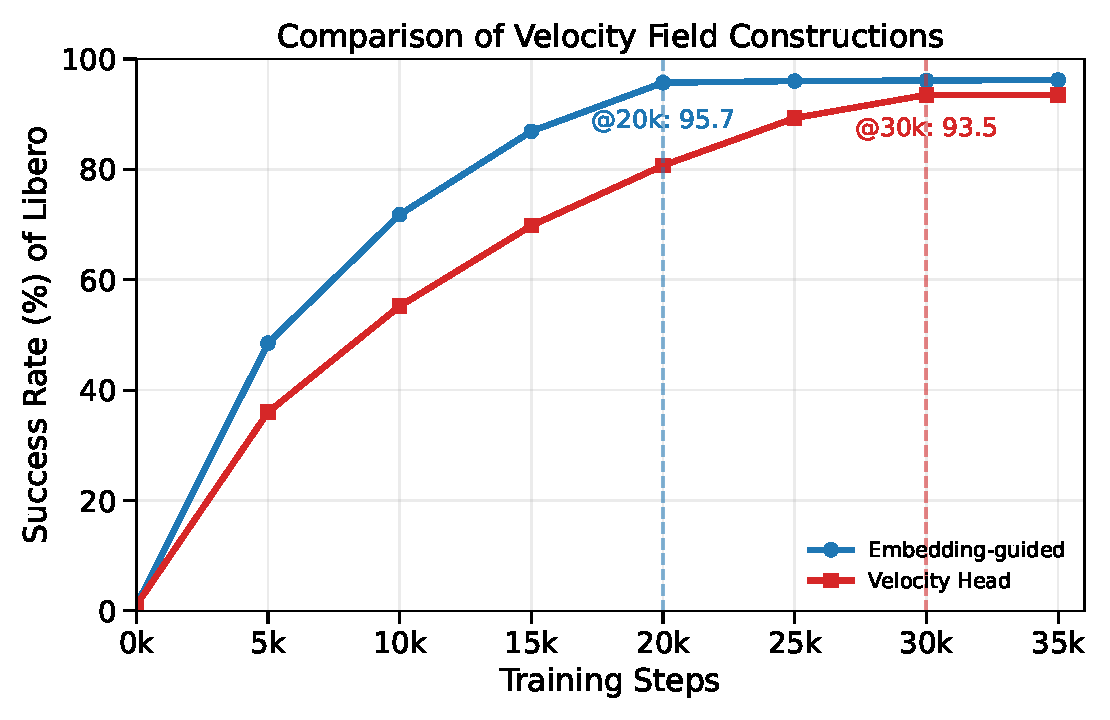
\includegraphics[width=0.8\linewidth]{figure/velocity_field_compare.pdf}
    \caption{Comparison of velocity field constructions across training steps. The Embedding-guided variant consistently outperforms the Velocity Head variant in both convergence speed and final performance, reaching a state-of-the-art success rate of 95.7\% on LIBERO with only 20k training steps.}
    \label{fig:velocity_field_compare}
\end{figure}
\subsection{Ablation Studies}
\label{sec:ablation}
We conduct ablation studies to isolate the effects of key design and training choices, including schedule hyperparameters $c$ and $\alpha$, two-stage decoding step allocation, and velocity-field construction. Detailed quantitative results are summarized in \Cref{tab:ablation_lambda_c_alpha,tab:ablation_two_stage,fig:velocity_field_compare}.


\begin{wraptable}{r}{0.48\textwidth}
    \vspace{-10mm}
    \centering
    \footnotesize
    \setlength{\tabcolsep}{4pt}
    \caption{Ablation study on $c$ and $\alpha$.}
    \label{tab:ablation_lambda_c_alpha}
    \begin{tabular}{c|c|c|c}
        \toprule
        $c$ & $\alpha$ & CALVIN $\uparrow$ & LIBERO (\%) $\uparrow$ \\
        \midrule
        1 & 1 & 4.38 & 95.0 \\
        3 & 1 & 4.44 & 95.7 \\
        5 & 1 & 4.40 & 95.2 \\
        3 & 0.5 & 4.40 & 95.6 \\
        \bottomrule
    \end{tabular}
    \vspace{-5mm}
\end{wraptable}

\paragraph{Effect of $c$ and $\alpha$.}
In Eq.~\ref{eq:beta_t}, $c$ controls the overall scale of $\beta_t$, while $\alpha$ controls the temporal curvature of the schedule, determining how quickly refinement concentrates as $t\!\to\!1$.
\Cref{tab:ablation_lambda_c_alpha} shows that \method~is robust to moderate changes of both parameters, with $c=3,\alpha=1$ giving the best  trade-off.
Under this setting, \method~achieves the  Avg. Len. of 4.44 on CALVIN and average success rate of 95.7\% on Libero. 
Increasing $c$ to 5 or decreasing $\alpha$ to 0.5 causes only minor fluctuations, indicating stable refinement dynamics across a reasonably wide hyperparameter region.

\begin{wraptable}{r}{0.5\textwidth}
    \vspace{-10mm}
    \centering
    \footnotesize
    \setlength{\tabcolsep}{5pt}
    \caption{Ablation on two-stage decoding step allocation with fixed total steps ($T_{\mathrm{fine}} + T_{\mathrm{val}} = 16$).}
    \label{tab:ablation_two_stage}
    \begin{tabular}{c | c | c |c}
        \toprule
        $T_{\mathrm{fine}}$ & $T_{\mathrm{val}}$ & CALVIN $\uparrow$ & LIBERO (\%) $\uparrow$ \\
        \midrule
        16 & 0  & 4.37 & 94.8 \\
        15 & 1  & 4.39 & 95.2 \\
        14 & 2  & \textbf{4.44} & \textbf{95.7} \\
        12 & 4  & 4.41 & 95.4 \\
        8  & 8  & 4.35 & 95.1 \\
        \bottomrule
    \end{tabular}
    \vspace{-3mm}
\end{wraptable}
\paragraph{Effect of Two-Stage Decoding.}
We further ablate how decoding steps are allocated between the iterative refinement stage ($T_{\mathrm{fine}}$) and the deterministic validation stage ($T_{\mathrm{val}}$). We keep the total number of steps fixed at 16 and report Avg. Len. of CALVIN ABCD$\rightarrow$D  and average success rate of LIBERO in \Cref{tab:ablation_two_stage}. As shown in the table, using only iterative refinement  ($T_{\mathrm{val}}=0$) yields weaker performance. Introducing a short validation stage improves both benchmarks, and $T_{\mathrm{fine}}=14, T_{\mathrm{val}}=2$ achieves the best overall trade-off. In contrast, allocating too many steps to the validation stage slightly hurts action quality, suggesting that excessive early greedy release reduces refinement flexibility. Therefore, we use $T_{\mathrm{fine}}=14$ and $T_{\mathrm{val}}=2$ in all experiments.



\paragraph{Comparison of Velocity Field Constructions.}
To further analyze the effect of velocity-field design, we compare the embedding-guided formulation with the head-based formulation across training steps. As shown in~\Cref{fig:velocity_field_compare}, the embedding-guided variant converges faster in the early stages of training and consistently reaches better final task performance. This trend indicates that embedding guidance provides more informative and smooth optimization signals, leading to both improved data efficiency and a stronger final policy.




\subsection{In-Depth Analysis}
\label{sec:analysis}

% \begin{wraptable}{r}{0.5\textwidth}
%     \vspace{-10mm}
%     \centering
%     \footnotesize
%     \setlength{\tabcolsep}{2pt}
%     \caption{Inference efficiency comparison across AR, DD and DFM on CALVIN ABCD$\rightarrow$D. DD and DFM use the same decoding steps (16).}
%     \label{tab:efficiency_main}
%     \begin{tabular}{lcc}
%         \toprule
%         Method & Avg. Len. $\uparrow$ & Speed $\uparrow$ \\
%         \midrule
%         AR & 4.18 & 50.2  \\
%         DD & 4.32 & 62.1  \\
%         DD + Adap. Cache & 4.27 & 118.3  \\
%         DFM & 4.42 & 60.2  \\
%         DFM + Adap. Cache & 4.40 & 121.0  \\
%         \bottomrule
%     \end{tabular}
%     \vspace{-6mm}
% \end{wraptable}
\paragraph{Effectiveness of Decoding Method.}

\begin{table*}[t]
    \centering
    \footnotesize
    \begin{minipage}[t]{0.47\textwidth}
        \centering
        \setlength{\tabcolsep}{2pt}
        \caption{Inference efficiency comparison across AR, DD, and DFM on CALVIN ABCD$\rightarrow$D. DD and DFM use the same decoding steps (16).}
        \label{tab:efficiency_main}
        \begin{tabular}{l|c|c}
            \toprule
            Method & Avg. Len. $\uparrow$ & Speed $\uparrow$ \\
            \midrule
            AR & 4.18 & 50.2  \\
            DD & 4.32 & 62.1  \\
            DD + Adap. Cache & 4.27 & 118.3  \\
            DFM & \textbf{4.42} & 60.2  \\
            DFM + Adap. Cache & 4.40 & \textbf{121.0}  \\
            \bottomrule
        \end{tabular}
    \end{minipage}\hfill
    \begin{minipage}[t]{0.47\textwidth}
        \centering
        \setlength{\tabcolsep}{2pt}
        \caption{Ablation on training data scale on CALVIN ABCD$\rightarrow$D . We compare three discrete VLA paradigms across data scales, with DD and DFM evaluated using the same number of decoding steps.}
        \label{tab:ablation_data_scale}
        \begin{tabular}{c|ccc}
            \toprule
            Data Fraction & AR & DD & DFM (Ours) \\
            \midrule
            10\%  & 1.71 & 2.84 & \textbf{3.21}   \\
            50\%  & 3.01 & 3.88 & \textbf{4.03}   \\
            100\% & 4.18 & 4.32 & \textbf{4.44}   \\
            \bottomrule
        \end{tabular}
    \end{minipage}
\end{table*}
We keep the architecture unchanged and compare AR, DD, and our method, while also validating the effectiveness of Adaptive Cache in inference.
Results in \Cref{tab:efficiency_main} show that \method~achieves the best action quality among the compared decoding strategies. With Adaptive Cache enabled, both DD and DFM obtain clear speedups, and \textit{DFM+Adaptive Cache} delivers the fastest decoding while maintaining strong performance. These results indicate that DFM provides a favorable quality--efficiency trade-off under matched decoding steps.

% \begin{wraptable}{r}{0.5\textwidth}
%     \vspace{-8mm}
%     \centering
%     \footnotesize
%     \setlength{\tabcolsep}{4pt}
%     \caption{Ablation on training data scale on CALVIN ABCD$\rightarrow$D (Avg. Len. $\uparrow$). We compare three discrete VLA paradigms across data scales, with DD and DFM evaluated using the same number of decoding steps.}
%     \label{tab:ablation_data_scale}
%     \begin{tabular}{c|ccc}
%         \toprule
%         Data Fraction & AR & DD & DFM (Ours) \\
%         \midrule
%         10\%  & 1.71 & 2.84 & 3.21   \\
%         50\%  & 3.01 & 3.88 & 4.03   \\
%         100\% & 4.18 & 4.32 & 4.44   \\
%         \bottomrule
%     \end{tabular}
%     \vspace{-7mm}
% \end{wraptable}
\paragraph{Effect of training data size.}
\Cref{tab:ablation_data_scale} shows that \method~consistently outperforms both autoregressive and discrete diffusion baselines across all data scales on CALVIN ABCD$\rightarrow$D.
At 10\% data, \method~ achieves an Avg. Len. of 3.21, outperforming AR at 1.71 and discrete diffusion at 2.84 by +1.50 and +0.37, respectively. It also remains the best at 50\% data with 4.03 and at 100\% data with 4.44, showing consistent gains as data scale increases.
These results indicate that DFM-VLA is particularly beneficial in low-data regimes while maintaining consistent advantages as training data scales up.



\subsection{Real World Experiment}
\begin{figure}[t]
    \centering
    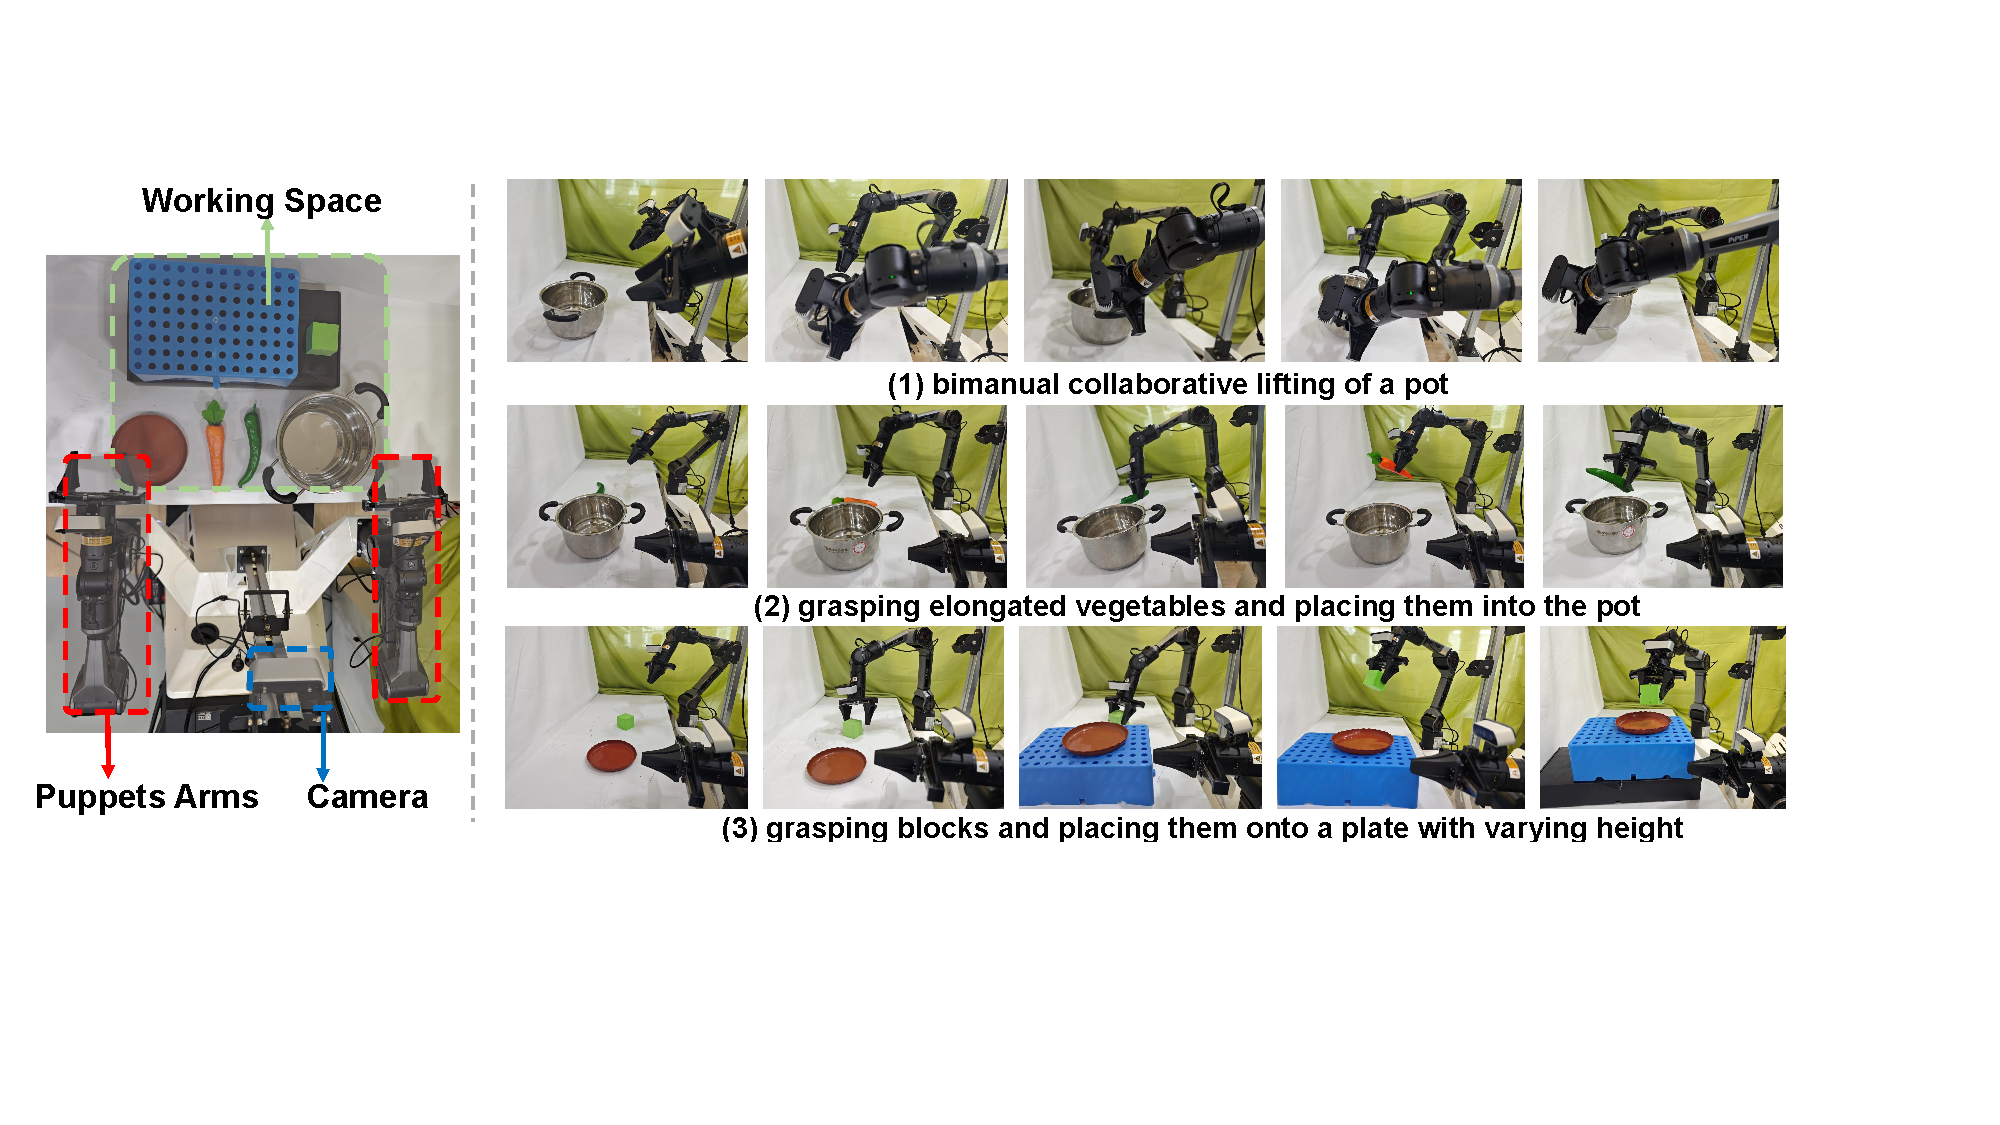
\includegraphics[width=0.99\linewidth]{figure/real_set.pdf}
    \caption{\textbf{Left:} The real-world robotic system for experiments.  \textbf{Right:} The representative task demonstrations.}

    \label{fig:real}
\end{figure}
%Setup.我们的真机实验在bimanual AgileX上进行，它具有两条机械臂，每条臂具有六个自由的的关节和一个夹爪。该机器具有三个摄像头：一个在机器中间高处视角，其余两个各自在机械臂的手腕上。
%Task Setting.我们一共设置了三个任务，如图所示，第一个任务是双臂协作举起锅；第二个是夹取条状蔬菜到锅中，蔬菜的位置和位姿会有所改变；第三个是夹取方块到盘子里，其中盘子的高度会进行改变。对于每个任务，我们均收集xx条数据进行训练，对于评估，我们对每个任务进行了四十次评估，记录他们的成功率以及完成速度。
\textbf{Setup.}
As shown in \Cref{fig:real}, 
we conduct real-world experiments on a bimanual AgileX platform equipped with two robotic arms, each with six degrees of freedom and a parallel gripper.
The system is instrumented with three RGB cameras: one fixed camera mounted at an elevated central viewpoint and two wrist-mounted cameras, one on each arm.

\noindent
\textbf{Task Setting.}
We design three representative manipulation tasks:
(1) bimanual collaborative lifting of a pot (\textit{Pot Lift});
(2) grasping elongated vegetables and placing them into the pot, where the object position and pose are varied (\textit{Place Veg. to Pot});
and (3) grasping a block and placing it onto a plate with varying height (\textit{Place Block to Plate}).
For each task, we collect 100 trajectories for training.
During evaluation, we run 40 trials per task and report both task success rate and completion speed.
\label{sec:real}

\noindent
\textbf{Results.}
We compare \method against representative methods from three action-generation paradigms for real-world manipulation: the autoregressive baseline $\pi_0$-FAST, the discrete diffusion baseline Dream-VLA, and the continuous diffusion baseline RDT~\citep{liu2024rdt}.
Table~\ref{tab:real_world_results} shows that \method~achieves the highest success rate on each task. Specifically, our \method~reaches a success rate of 77.5\% on \textit{Pot Lift}, which requires precise bimanual coordination; 70.0\% on \textit{Place Veg. to Pot}, which tests generalization to object positions and poses; and 65.0\% on \textit{Place Block to Plate}, which emphasizes spatial precision under varying plate heights. Overall, the average success rate of~\method~is 70.8\%, which surpasses RDT at 60.0\% by 10.8 percentage points and Dream-VLA at 54.2\% by 16.6 percentage points.

This result demonstrates that traditional discrete baselines (i.e., $\pi_0$-FAST and Dream-VLA) are weaker than the continuous diffusion baseline RDT because wrongly decoded action tokens cannot be refined, leading to error accumulation. 
In contrast, our method uses refined action guided by velocities over discrete action tokens to correct errors in time.
Meanwhile, its unified discrete input-output space better preserves semantic understanding from autoregressive VLM backbones~\citep{liang2025discrete,wen2025dvla}, yielding the best overall performance.
These results further show that action refinement with discrete flow matching remains highly competitive and robust in real-world settings.

\begin{table}[t]
    \centering
    \footnotesize
    \setlength{\tabcolsep}{3pt}
    \caption{Real-world success rate comparison (\%) on three tasks.}
    \label{tab:real_world_results}
    \begin{tabular}{lccc|c}
        \toprule
        Method & Pot Lift & Place Veg. to Pot & Place Block to Plate & Average \\
        \midrule
        $\pi_0$-FAST~\citep{pertsch2025fast} & 50.0 & 42.5 & 35.0 & 42.5 \\
        Dream-VLA~\citep{yedreamVLA} & 57.5 & 62.5  & 42.5  & 54.2 \\
        RDT~\citep{liu2024rdt} & 65.0 & 62.5  & 52.5  & 60.0 \\
         \rowcolor[gray]{0.9}
        \textbf{\method+Head} & 70.0 & 67.5  & 60.0 & 65.8 \\
        \rowcolor[gray]{0.9}
        \textbf{\method+Embed} & \textbf{77.5}  & \textbf{70.0} & \textbf{65.0} & \textbf{70.8} \\
        \bottomrule
    \end{tabular}
\end{table}





\section{Conclusion}

In this paper, we present \method, a discrete flow-matching VLA framework that enables iterative full-sequence action refinement through token-level velocity modeling. Our \method~can revisit and correct previously generated action tokens, improving action consistency for robotic manipulation.
We further study two complementary velocity-field constructions and integrate a practical two-stage decoder. Extensive experiments demonstrate that \method~consistently delivers strong action quality while maintaining high inference efficiency.


% In this paper, we presented \method, a discrete flow matching framework for the VLA model that enables iterative full-sequence action refinement. Unlike autoregressive and discrete diffusion baselines, our \method~revisits and selectively updates action tokens through token-level velocity modeling, thereby improving action consistency in robotic manipulation.

% Our approach explores two velocity-field constructions: an embedding-guided formulation that defines structured probability paths and an auxiliary velocity head formulation that predicts velocities directly from hidden states. It further integrates kinetic-optimal velocity design with a practical two-stage decoder that couples iterative refinement and deterministic validation, achieving superior execution quality and favorable inference efficiency across CALVIN, LIBERO, and real-world evaluations.

% \textbf{Future work.} 
% Future work includes scaling DFM-based VLA pretraining, improving  token refinement, and extending the framework to tighter joint modeling of perception, reasoning, and action in more open-ended real-world environments.





% ---- Bibliography ----
%
% BibTeX users should specify bibliography style 'splncs04'.
% References will then be sorted and formatted in the correct style.
%


% \section{Acknowledgments}

% \clearpage
% \newpage
\bibliographystyle{assets/plainnat}
\bibliography{paper}

\clearpage
\newpage
\onecolumn
\beginappendix
\renewcommand{\thefigure}{S\arabic{figure}}
\renewcommand{\thetable}{S\arabic{table}}
\setcounter{figure}{0}
\setcounter{table}{0}


\section{Training Pipeline}
\label{sec:training_pipeline}

\paragraph{Action-modality training.}

Following the notation in the main manuscript, we denote the discretized instruction and observations as $l$, and apply noising and prediction only to the action modality. 
As shown in \Cref{alg:action_dfm_training},
let $x_1=[x_1^1,\ldots,x_1^D]$ be the clean action token sequence. At each training iteration, we sample $t\sim\mathcal{U}(0,1)$, draw corrupted action tokens $x_t\sim p_t(\cdot\mid x_1)$ from the prescribed probability path, and feed $(x_t, l)$ into the predictor to obtain per-position distributions $p_{1|t}^{\theta}(\cdot\mid x_t, l)$. The model refines all action tokens in parallel.

The training objective follows the same definitions in the main manuscript. Depending on the velocity modeling variant, we optimize either $\mathcal{L}_{\text{ce}}$ or $\mathcal{L}_{\text{head}}$.
% ; optionally, we use a weighted joint objective $\mathcal{L}_{\text{train}}=\mathcal{L}_{\text{ce}}+\mu\mathcal{L}_{\text{head}}$.

\begin{algorithm}[t]
\caption{Action-Modality DFM Training}
\label{alg:action_dfm_training}
\begin{algorithmic}[1]
\REQUIRE Predictor $p_\theta$, learning rate $\eta$, optional weight $\mu$
\REPEAT
    \STATE Sample $(l,x_1)\sim p_{\text{data}}$
    \STATE Sample $t\sim\mathcal{U}(0,1)$
    \STATE Sample $x_t\sim p_t(\cdot\mid x_1)$
    \STATE Choose $\mathcal{L}_{\text{train}}\in\{\mathcal{L}_{\text{ce}},\mathcal{L}_{\text{head}}\}$
    \STATE Compute $\mathcal{L}_{\text{train}}$ from $(x_t,l)$ and $x_1$
    \STATE $\theta\leftarrow\theta-\eta\nabla_\theta\mathcal{L}_{\text{train}}$
\UNTIL{converged}
\STATE \textbf{return} trained predictor $p_\theta$
\end{algorithmic}
\end{algorithm}

\section{Visualization of Refinement Process}
\label{sec:space_visualization}

To provide intuition for the action-embedding-guided velocity modeling in the main manuscript, \Cref{fig:space} visualizes a token refinement trajectory in the embedding space at three representative times ($t=0$, $t=0.5$, and $t=1$). The hollow blue circles denote candidate token IDs, the red point denotes the predicted clean token $x_1^{\mathrm{pred}}$, and $x_t$ denotes the current token state.

At each step, the transition rate favors destinations that are closer to $x_1^{\mathrm{pred}}$ than the current token. As a result, tokens within the jumpable range can be selected, and candidates nearer to $x_1^{\mathrm{pred}}$ receive higher jump probability (deeper red). As refinement proceeds, $x_t$ moves toward $x_1^{\mathrm{pred}}$, the feasible jump set becomes progressively smaller, and updates become increasingly local. This behavior illustrates how DFM-VLA balances early exploration with late-stage stabilization during iterative action refinement.

\begin{figure}[t]  
    \centering
    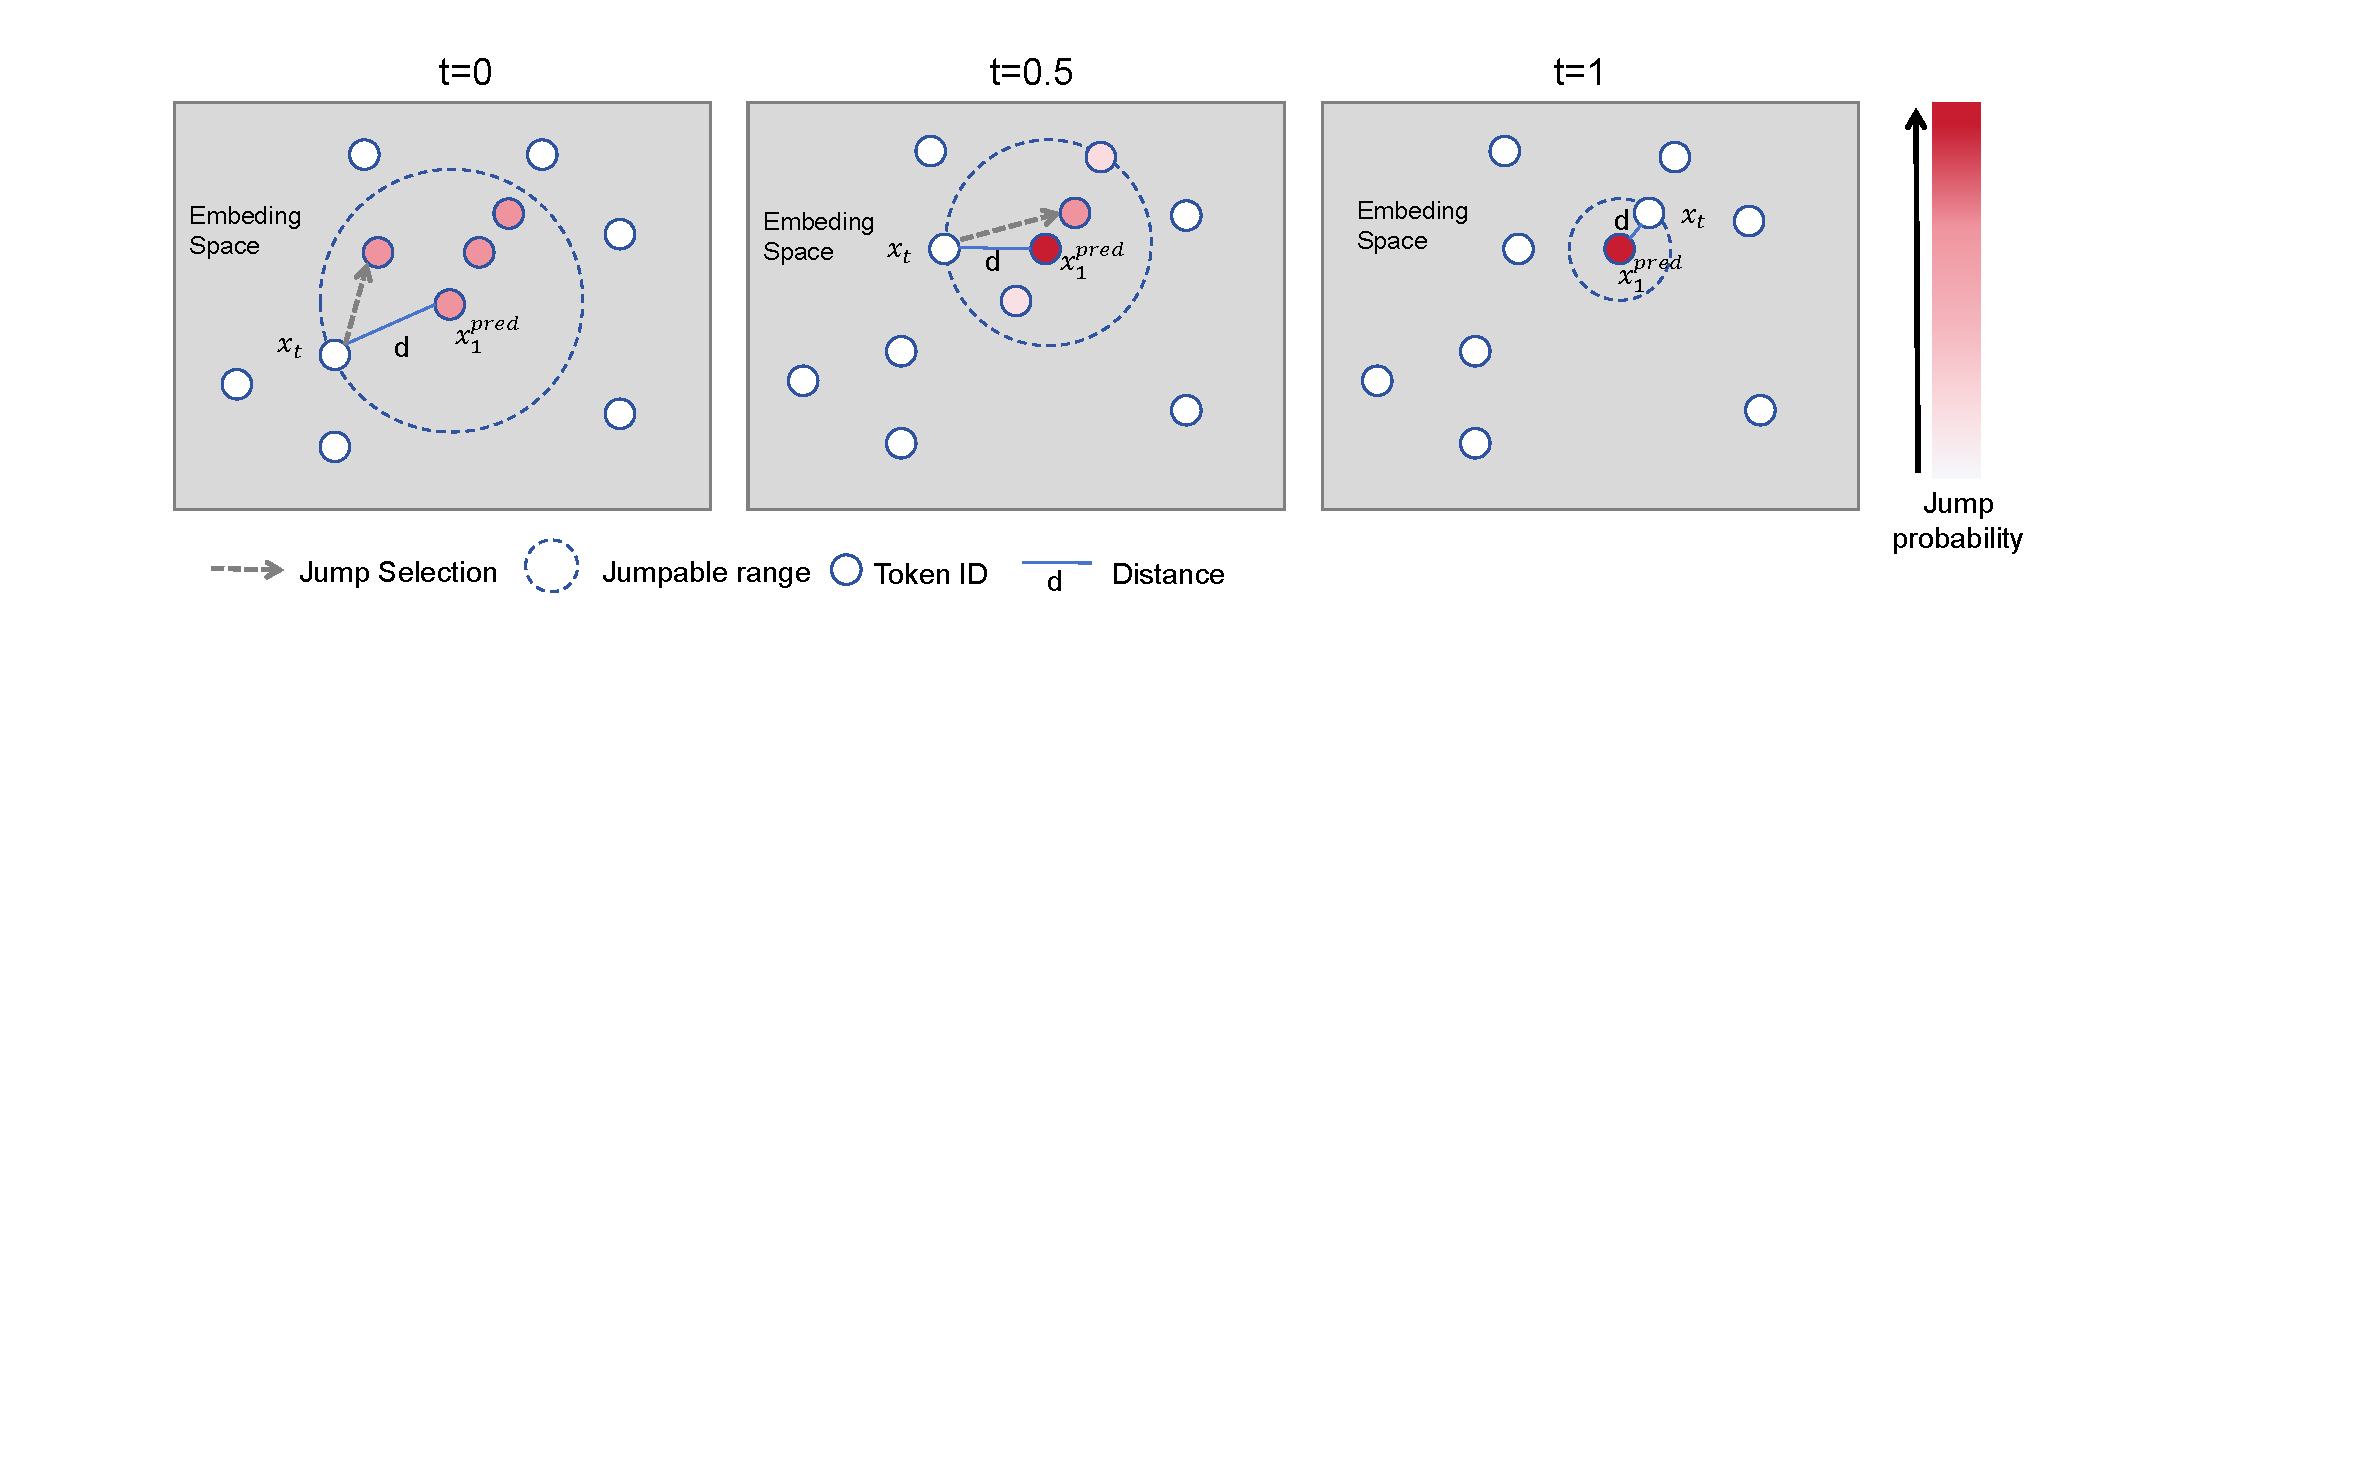
\includegraphics[width=0.98\linewidth]{figure/space.pdf} 
    \caption{Embedding-space view of iterative refinement. From $t=0$ to $t=1$, the current token $x_t$ progressively moves toward $x_1^{\mathrm{pred}}$, while transition probabilities increasingly concentrate around the target.}
    \label{fig:space} 
\end{figure}

\section{Implementation Hyperparameters}
\label{sec:implementation_hparams}

\Cref{tab:impl_hparams} summarizes the launch and training hyperparameters used in our implementation.

\begin{table}[t]
\centering
\small
\caption{Implementation hyperparameters for training.}
\label{tab:impl_hparams}
\begin{tabular}{p{0.45\linewidth}p{0.47\linewidth}}
\toprule
\textbf{Parameter} & \textbf{Value} \\
\midrule
\texttt{nproc\_per\_node} & \texttt{8} \\
\texttt{nnodes} & \texttt{1} \\
% \texttt{node\_rank} & \texttt{\$\{RANK\}} \\
% \texttt{master\_addr} & \texttt{\$\{MASTER\_ADDR\}} \\
% \texttt{master\_port} & \texttt{\$\{MASTER\_PORT\}} \\
% \texttt{train script} & \texttt{train/train\_moe.py} \\
% \texttt{model\_name\_or\_path} & \texttt{\$\{MODEL\_PATH\}} \\
% \texttt{model\_config\_path} & \texttt{configs/moe\_fast\_video.json} \\
% \texttt{deepspeed} & \texttt{scripts/sft/zero3.json} \\
% \texttt{output\_dir} & \texttt{logs/libero/\$\{EXP\_NAME\}} \\
% \texttt{data\_path} & \texttt{\$\{DATAPATH\}} \\
% \texttt{action\_tokenizer\_path} & \texttt{\$\{ACTION\_TOKENIZER\_PATH\}} \\
\texttt{learning\_rate} & \texttt{8e-5} \\
\texttt{min\_learning\_rate} & \texttt{5e-6} \\
\texttt{lr\_scheduler\_type} & \texttt{cosine\_with\_min\_lr} \\
\texttt{warmup\_steps} & \texttt{50} \\
\texttt{weight\_decay} & \texttt{0.1} \\
\texttt{max\_grad\_norm} & \texttt{5.0} \\
\texttt{adam\_beta1} / \texttt{adam\_beta2} & \texttt{0.9} / \texttt{0.95} \\
\texttt{adam\_epsilon} & \texttt{1e-6} \\
\texttt{bf16} / \texttt{tf32} & \texttt{True} / \texttt{True} \\
\texttt{max\_steps} & \texttt{16000} \\
% \texttt{per\_device\_train\_batch\_size} & \texttt{6} \\
\texttt{gradient\_accumulation\_steps} & \texttt{4} \\
\texttt{effective global batch size} & \texttt{8 * NGPUS * 4} \\
% \texttt{dataloader\_num\_workers} & \texttt{16} \\
% \texttt{gradient\_checkpointing} & \texttt{True} \\
% \texttt{frames} / \texttt{action\_frames} & \texttt{1} / \texttt{10} \\
% \texttt{max\_position\_embeddings} & \texttt{1370} \\
% \texttt{null\_prompt\_prob} & \texttt{0.15} \\
% \texttt{seed} & \texttt{42} \\
% \texttt{logging\_steps} & \texttt{20} \\
% \texttt{save\_strategy} / \texttt{save\_steps} & \texttt{steps} / \texttt{6000} \\
% \texttt{eval\_strategy} & \texttt{no} \\
% \texttt{apply\_loss\_on\_only\_vision} & \texttt{False} \\
% \texttt{apply\_loss\_on\_only\_action} & \texttt{True} \\
% \texttt{actions} / \texttt{actions\_format} & \texttt{True} / \texttt{fast} \\
% \texttt{use\_gripper} & \texttt{True} \\
% \texttt{video\_format} & \texttt{interleave} \\
\bottomrule
\end{tabular}
\end{table}
% \newpage




\end{document}
